\chapter{Grundlagen}
\label{cha:grundlagen}

Die Vernetzung aller Dinge wurde visionär bereits 1926 von Nikola Tesla \parencite{jeschke2017industrial} vorhergesagt. 

\begin {quote} \textit{``When wireless is perfectly applied, the whole earth will be converted into a huge brain, which in fact it is, all things being particles of a real and rhythmic whole. A man will be able to carry one in his vest pocket.''} \end{quote}

Dieses Kapitel definiert die Begriffe Industrie 4.0, Cloud Computing, Internet of Things und Siemens MindSphere.

\section{Industrie 4.0}

Der Begriff \textit{Industrie 4.0} wurde zum ersten Mal 2011 auf der "`Messe Hannover"' verwendet \parencite{jeschke2017industrial}. Er soll andeuten, dass es sich hier um die vierte industrielle Revolution handelt, welche die Arbeitswelt und Gesellschaft genauso nachhaltig verändern wird wie die drei vorangegangenen Revolutionen.

\subsection{Historie von Industrie 4.0}

\subsubsection{Erste industrielle Revolution}
Die \textit{erste industrielle Revolution} im 18. Jahrhundert wurde durch die Erfindung der Dampfmaschine (siehe Abb.~\ref{fig:Dampfmaschine}) und die Nutzung von Wasser- und Dampfkraft bzw. durch die Einführung mechanischer Produktionsanlagen eingeleitet \parencite{andelfinger2017industrie}. Vorausgegangen waren eine verstärkte Urbanisierung der Bevölkerung und die Verfügbarkeit von Rohstoffen wie Kohle und Eisen in großen Mengen. Erstmals konnte mit Hilfe von Maschinen dem Menschen ein Teil der körperlich schweren Arbeit abgenommen werden. Somit war es nun möglich, bedeutend schneller und in größeren Stückzahlen zu produzieren. Eine erste Form der industriellen Produktion bzw. Industrialisierung war entstanden.


\begin{figure}%[H]
\centering
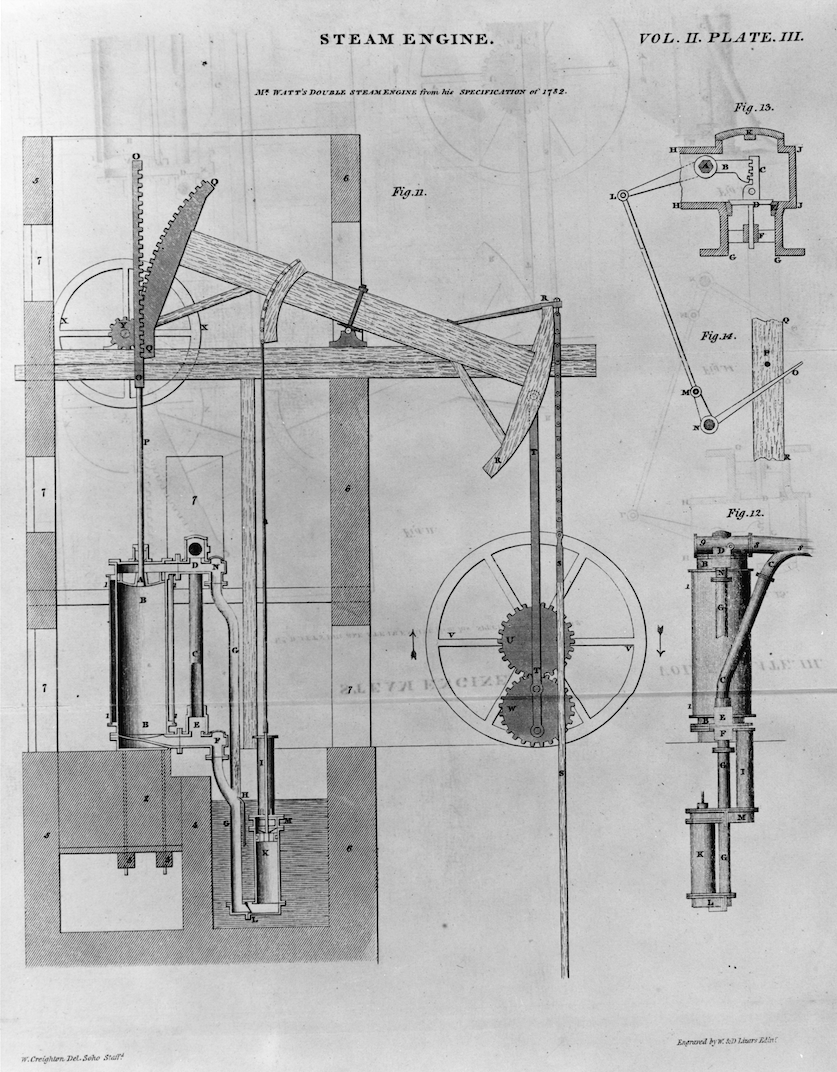
\includegraphics[width=.45\textwidth]{dampfmaschine.png} 
\caption{Dampfmaschine um 1822 \cite{SteamEngin1822}.}
\label{fig:Dampfmaschine}
\end{figure}

\subsubsection{Zweite industrielle Revolution}
Ende des 19. Jahrhunderts wurde damit begonnen, die industrielle Produktion in ihre Teilaufgaben und einzelnen Fertigungsschritte zu zerlegen \parencite{andelfinger2017industrie}. Diese Entwicklung, eng mit den Begriffen \textit{Taylorismus}\footnote{Taylorismus benannt nach dem US-Amerikaner Frederick Winslow Taylor (1856-1915).} und \textit{Fordismus}\footnote{Fordismus benannt nach dem US-amerikanischen Industriellen Henry Ford (1863-1947).} verbunden, erreichte eine weitere Steigerung der Stückzahlen durch die Prozesssteuerung von Arbeitsabläufen.

Der \textit{Taylorismus} verfolgt drei miteinander verbundene Ziele (nach Bonazzi \parencite{bonazzi2014geschichte}):

\begin{itemize}
\item Zentralisierung und Rationalisierung der Weisungsbefugnisse
\item Erhöhung der Produktion und der Leistungsfähigkeit der Arbeiter und der Maschinen durch Reorganisation
\item Nutzung der Wissenschaft zur Betriebsführung durch Normierung von Arbeitsobjekten, Arbeitszeit und Arbeitstätigkeit
\end{itemize}

Während im Taylorismus die Aufmerksamkeit vor allem auf die Organisation der Fabrikarbeit gerichtet wird, konzentriert sich das Konzept des \textit{Fordismus} auf die Größendimension der Produktionseinheiten und die Massenproduktion standardisierter Güter \parencite{bonazzi2014geschichte}. Im Vordergrund steht die Massenproduktion, die durch Starrheit des Produktionsprozesses bzw. durch homogene Produkte charakterisiert wird. 

Auch weniger gut ausgebildete Arbeitskräfte konnten eingesetzt werden, weil jeweils nur ein einzelner Fertigungsschritt der Produktion beherrscht werden mussten. In dieser Zeit entstanden die ersten Fließbandproduktionen (siehe Abb.~\ref{fig:Fliessbandanlage}) und auch die Umstellung auf arbeitsteilige Massenproduktion bzw. Rationalisierung erfolgte \parencite{hocker2015}.

\begin{figure}%[H]
\centering
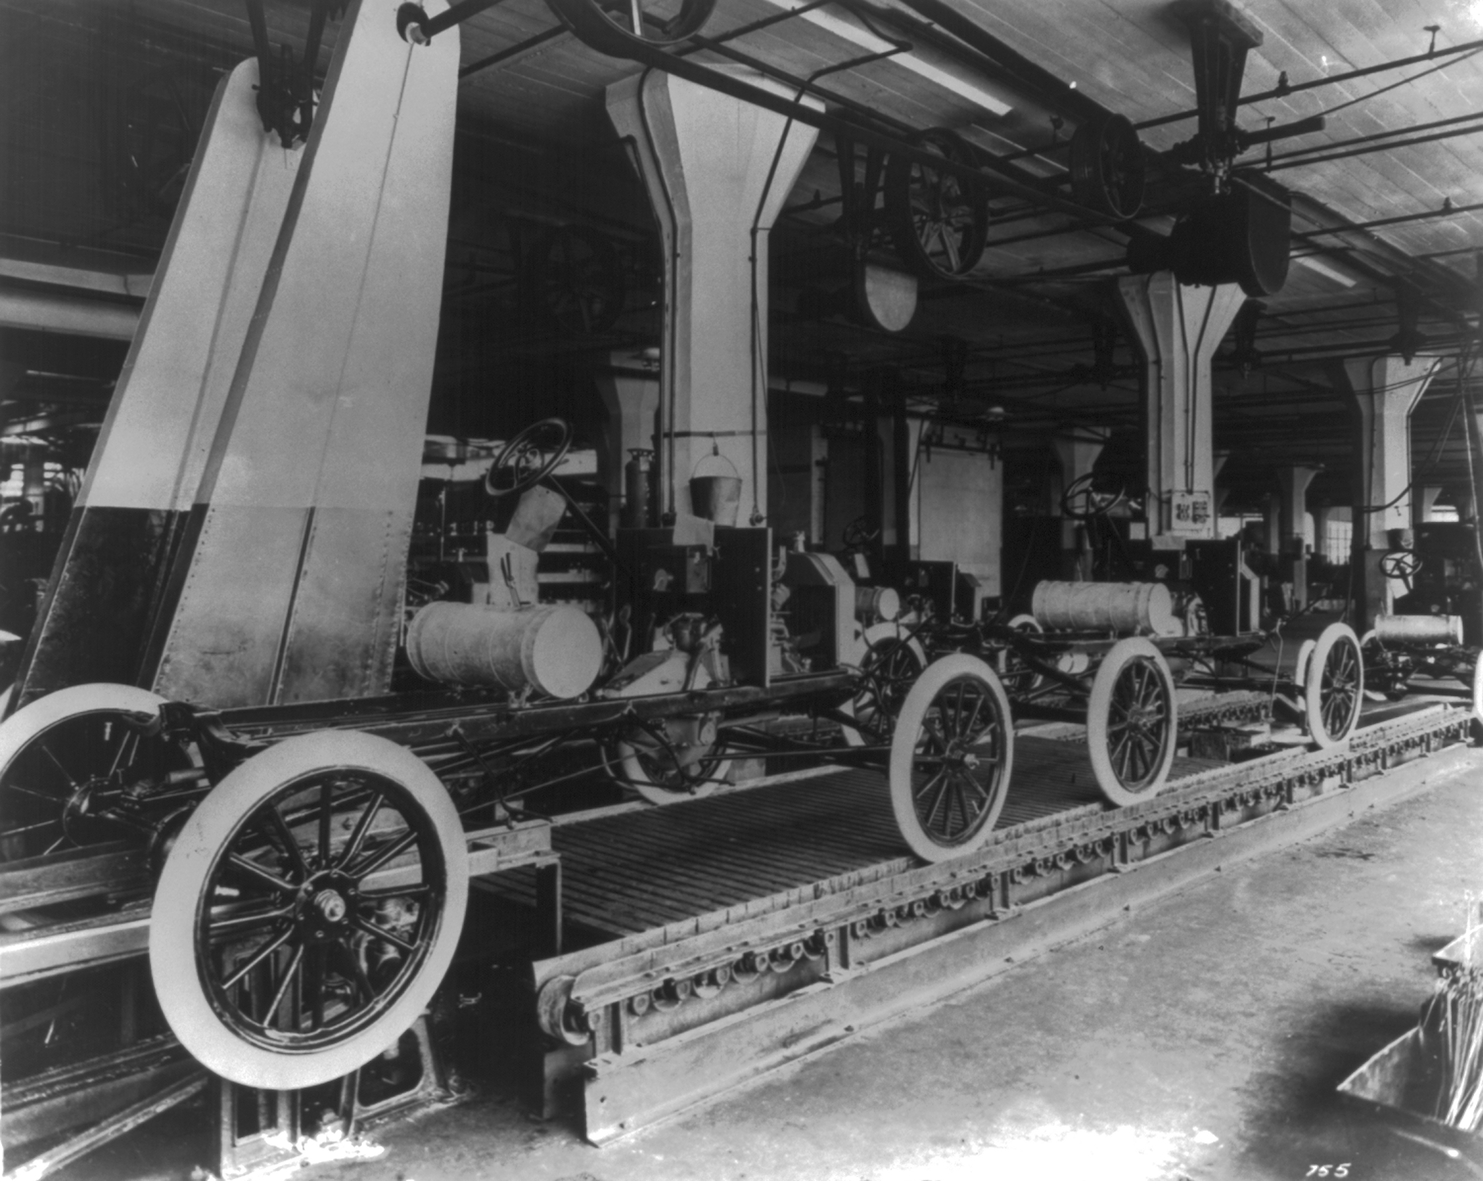
\includegraphics[width=.65\textwidth]{fordFliessband.png} 
\caption{Fließbandanlage Ford Motor Company's Highland Park im Jahr 1913 \cite{FordAssemblyLine1913}.}
\label{fig:Fliessbandanlage}
\end{figure}

\subsubsection{Dritte industrielle Revolution}
Die nächste einschneidende Änderung in der Industrie erfolgte durch den Einsatz von elektronischen Systemen ab Mitte des 20. Jahrhunderts \parencite{andelfinger2017industrie}. Durch den Einsatz von Elektronik und Informationstechnologie (siehe Abb.~\ref{fig:Computeranlage}) waren eine weitere Automatisierung der Produktion und Prozessoptimierungen möglich. Diese Neuerungen führten dazu, dass viele der körperlich schweren oder gefährlichen Arbeiten durch Maschinenanlagen übernommen wurden. Außerdem wurde dadurch eine konstante und höhere Qualität in der Produktion erreicht. Diese Entwicklung wird auch als Informatisierung bzw. Automatisierung bezeichnet \parencite{hocker2015}. 

\begin{figure}%[H]
\centering
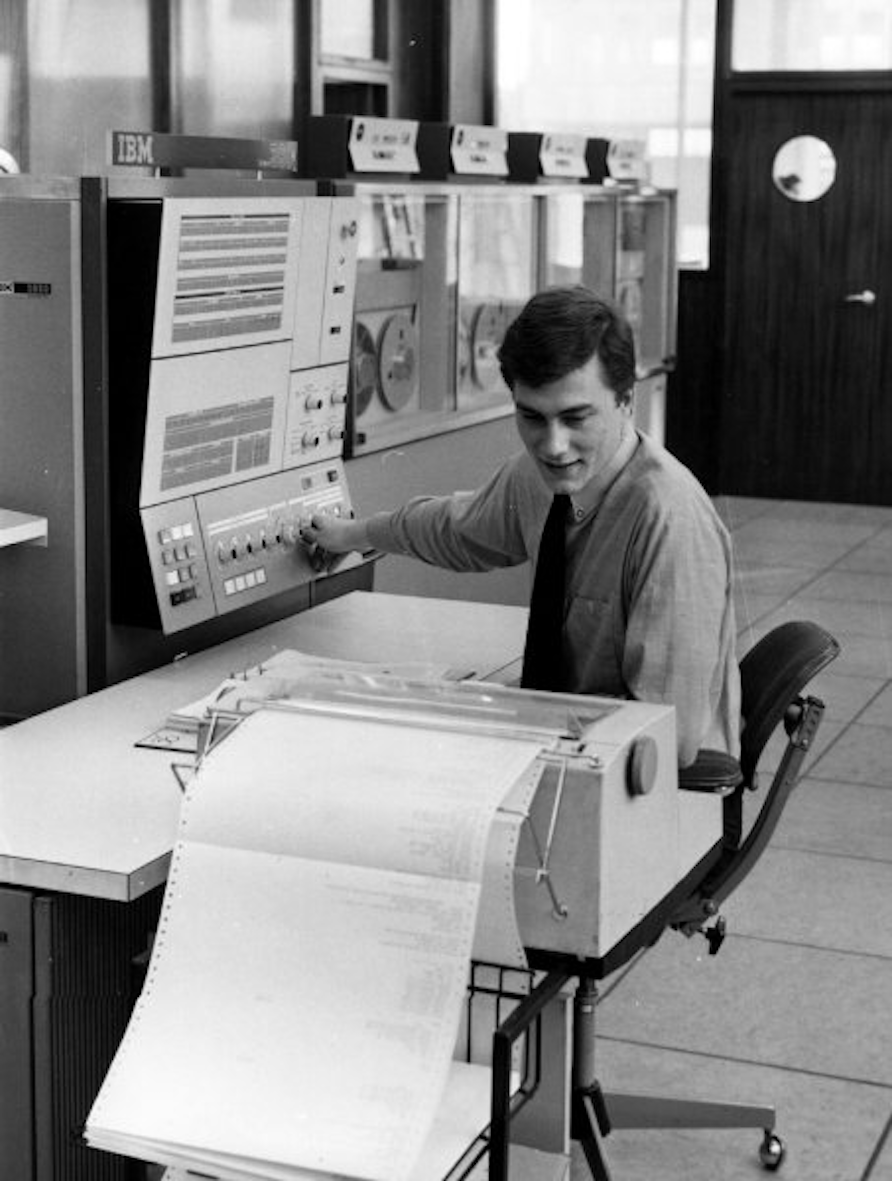
\includegraphics[width=.45\textwidth]{computerRev3.png} 
\caption{Computeranlage aus den 1970er-Jahren \cite{Spiegel}.}
\label{fig:Computeranlage}
\end{figure}

\subsubsection{Industrie 4.0}
Während in der Phase der dritten industriellen Revolution noch jede Betriebsanlage für sich stand und einer zentralisierten Kontrolle unterlag, wird bei der Umsetzung von \textit{Industrie 4.0} der gesamte Lebenszyklus eines Produkts berücksichtigt \parencite{andelfinger2017industrie}. Ein sogenanntes End-To-End-Design wird umgesetzt. Menschen, Dinge und Systeme sind miteinander verbunden und schaffen eine totale Vernetzung. Dadurch entstehen optimierte Wertschöpfungsketten und -netzwerke. 

Ein Integrationskonzept für die Informationsverarbeitung in Produktionsunternehmen vereinigt ein \acl{PPS} mit \acl{CAD} und \acl{CAM}. Cyber-physische Systeme und \acl{M2M}-Kommunikation sind dabei Grundkomponenten. Ein Cyber-physisches System besteht aus mechanischen, elektronischen und softwaretechnischen Komponenten. 

In Abbildung~\ref{fig:AutomotiveShowcase} sieht man eine interaktive Messe- und Ausstellungsapplikation der Firma Siemens Graphscape: "`Siemens Future Forum Industrie 4.0 Automotive Showcase"' als Beispiel, wie eine Produktionsstätte im System Industrie 4.0 organisiert sein kann.

\begin{figure}%[H]
\centering
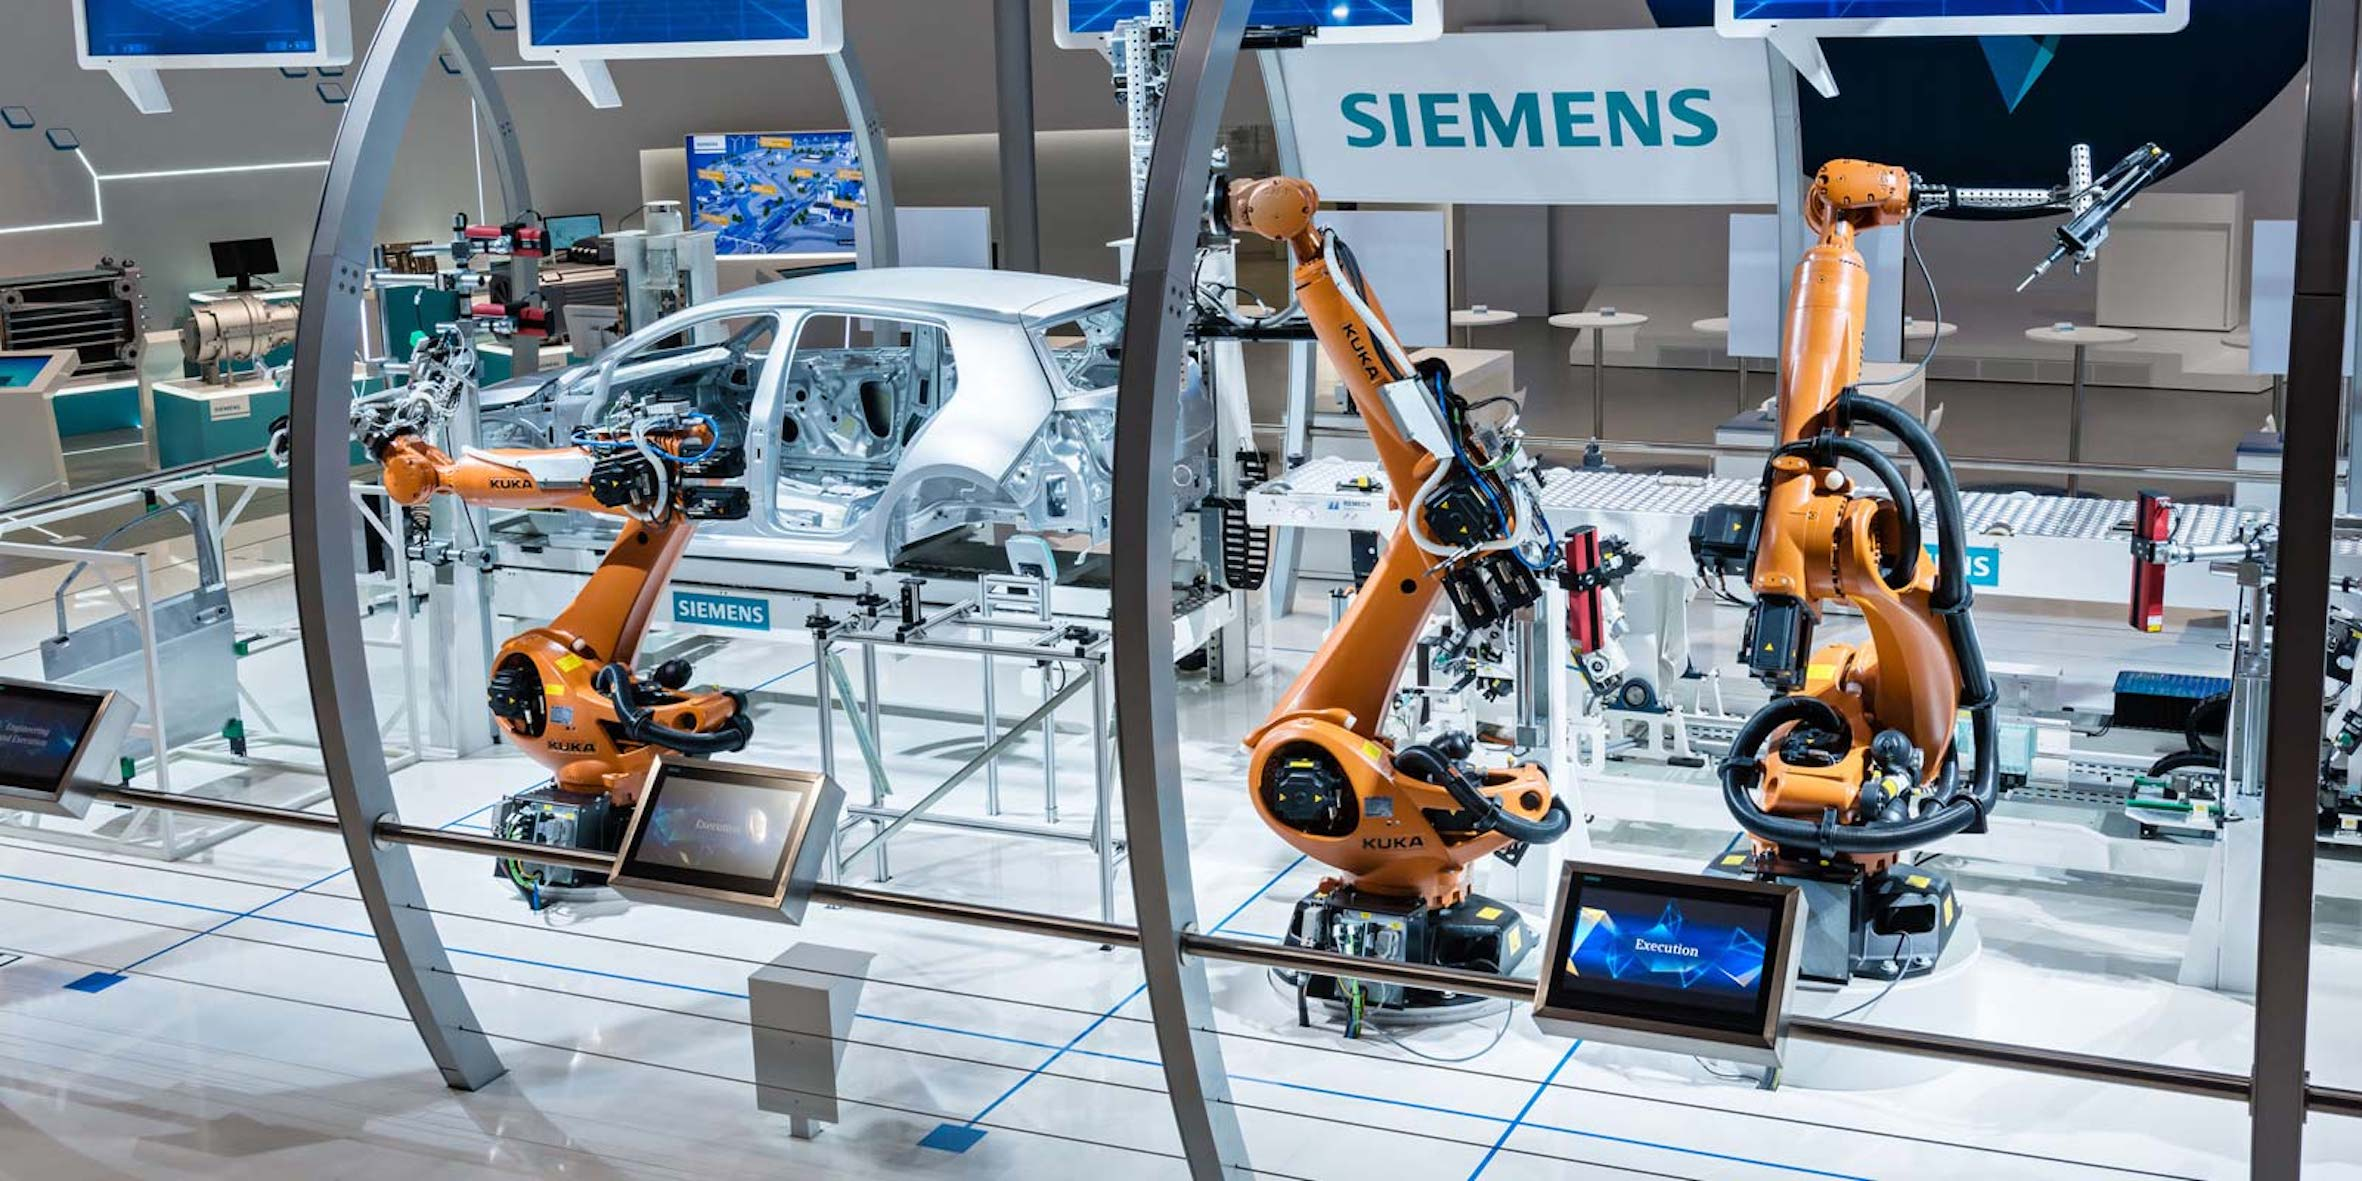
\includegraphics[width=1\textwidth]{siemens_automotive_1.jpg} 
\caption{Siemens Future Forum Industrie 4.0 Automotive Showcase \cite{Siemens}.}
\label{fig:AutomotiveShowcase}
\end{figure}

Industrie 4.0 und \acl{IIoT} sind in den letzten Jahren zu Hauptkonzepten der Industrie geworden und haben weiterhin großes Potential \parencite{gilchrist2016industry}.

\subsection{Hauptcharakteristika und Designprinzipien von Industrie 4.0}
\paragraph{Es gibt folgende vier Hauptcharakteristika von Industrie 4.0 (nach Gilchrist \parencite{gilchrist2016industry}):}
\begin{itemize}
\item vertikale Integration von intelligenten Produktionssystemen:\\
Alle Prozessschritte der Wertschöpfungskette greifen optimal ineinander. Nur so kann auf Ereignisse wie Änderung der Nachfrage oder des Lagerbestands oder  Maschinendefekte rasch reagiert werden. Die vertikale Integration erleichtert auch die kundenspezifische Produktion. 
\item horizontale Integration durch globale Wertschöpfungsnetzwerke:\\
Dies beschreibt das Zusammenspiel der verschiedenen Prozesse der jeweils logischen Ebene -- übergreifend auch auf Partner und Kunden.
\item Einbezug aller Bereiche der Wertschöpfungskette:\\
Der komplette Lebenszyklus eines Produkts von der Herstellung bis zur Entsorgung wird hier betrachtet. Der Fokus liegt dabei auf der Kundenzufriedenheit, erzielt durch Produkte von hoher Qualität.
\item Beschleunigung bzw. Optimierung der Herstellung:\\
Auch bei Industrie 4.0 bleibt dies weiterhin ein unternehmerisches Hauptziel.
\end{itemize}
\vspace{\baselineskip}

\paragraph{Zusätzlich zu den Hauptcharakteristika gibt es noch folgende sechs Designprinzipien für die Umsetzung von Industrie 4.0 (nach Gilchrist \parencite{gilchrist2016industry}):}
\begin{itemize}
\item Interoperabilität zwischen Mensch, intelligenter Fabrik und Technologien:\\
Ein Produktionsprozess verfolgt nicht nur einen gewissen Ablauf, sondern durch Interoperabilität finden ständig Interaktionen zwischen allen Projektpartnern statt. 
\item Virtualisierung (virtueller Zwilling):\\
Eine Virtualisierung der physischen Welt ermöglicht ein einfacheres Modifizieren und Testen des Systems ohne die physischen Prozesse zu beeinträchtigen.
\item Dezentralisierung:\\
Dies erlaubt einzelnen Systemen autonome Entscheidungen innerhalb einer intelligenten Fabrik zu treffen.
\item Echtzeit-Umsetzung:\\
Eine Echtzeit-Umsetzung in Industrie 4.0 umfasst sowohl das Sammeln der Daten als auch das Feedback und das Überwachen der Prozesse.
\item Schwerpunktsetzung auf Service:\\
Interne und externe Services sind in intelligenten Fabriken erforderlich; die Bereitstellung dieser Services wird von Gilchrist als \textit {Schwerpunktsetzung auf Service} bezeichnet \parencite{gilchrist2016industry}.
\item Modularisierung:\\
Um eine möglichst hohe Flexibilität für rasche Anpassung an Veränderungen zu erreichen, sollte bei der Strukturierung auf Modularisierung geachtet werden. Zusätzlich erleichtert dies die Kapselung einzelner Bereiche und die Datenabstraktion.
\end{itemize}
\vspace{\baselineskip}
War es in den 1990er und 2000er-Jahren noch unmöglich, Daten in den erforderlich großen Mengen zu speichern -- weil es einerseits zu teuer und andererseits die Rechenleistung für eine Analyse noch nicht vorhanden war -- ist dies mittlerweile durch Cloud Computing und industrielles Internet möglich. Zusätzlich hat auch die Entwicklung von Smartphones mit Internetzugang rund um 2007 die Entwicklung von Industrie 4.0 weiter vorangetrieben \parencite{gilchrist2016industry}.

\subsection{Ziele von Industrie 4.0}
Ein Ziel von Industrie 4.0 ist es, die Informationstechnik in die Produktion sowie in Produkte und Dienstleistungen zu integrieren \parencite{reinhart2017handbuch}. Dies geschieht durch mehrere Faktoren: 

\begin{itemize}
\item intelligente Fabriken:\\
Im Bereich der Produktion werden intelligente Fabriken entwickelt \parencite{vogel2017handbuch}. Hierbei werden Anlagen mit Sensorik ausgestattet und vernetzt. Durch die intelligente Fabrik sind in der Folge auch intelligente Operationen wie flexible Produktionsplanung und Produktionssteuerung möglich. Zusätzlich gibt es in Industrie 4.0 auch intelligente Produkte, welche auch nach dem Verkauf mit dem Hersteller in Verbindung stehen und datengetriebene Leistungen durch die Vernetzung von Hersteller, Produkt und Kunde bieten.

\item unternehmerische Ziele:\\
Die unternehmerischen Ziele sind hierbei die Effizienzsteigerung durch weitere Automatisierung, kundenindividuelle Produkte zu Kosten eines Massenprodukts, Steigerung des Umsatzes durch digital veredelte Produkte und die Erschließung neuer Märkte \parencite{reinhart2017handbuch}. In einem Industrie 4.0 Unternehmen wird vorausschauend produziert und die Produktion passt sich automatisch an.
\end{itemize}
\vspace{\baselineskip}

Um die Umsetzung von Industrie 4.0 gewinnbringend realisieren zu können, müssen Voraussetzungen in unterschiedlichen Bereichen wie z.B. Organisation, Produktion, Produkte und Services erfüllt werden: 
\begin{itemize}
\item Produktion:\\
In der Produktion muss \ac{IT} eingesetzt werden und eine digitale Repräsentation der Anlagenteile bzw. Assets erfolgen. Die IT-Infrastruktur muss die Daten sammeln und speichern. Danach muss eine Datenanalyse erfolgen, um daraus Erkenntnisse zu gewinnen.

\item Daten:\\
Werden Daten in so großen Mengen gesammelt, dass diese  mit herkömmlichen Datenbanksystemen und Werkzeugen nicht ohne Weiteres verarbeitet werden können, spricht man von \textit{Big Data} \parencite{gilchrist2016industry}. Zusätzlich zur Menge erschwert die große Diversität der Daten die Analyse und auch die Visualisierung. Eine weitere Herausforderung ist es, Daten zu verarbeiten, welche ständig durch neue Einspeisung von Sensordaten vergrößert werden \parencite{stackowiak2015big}. 

\item MitarbeiterInnen:\\
Um den Anforderungen zu entsprechen und die Ziele von Industrie 4.0 zu erreichen müssen die Mitarbeiter eines Unternehmens entsprechend geschult werden und das Informationsmanagement muss im Unternehmen akzeptiert werden.
\end{itemize}
\vspace{\baselineskip} 

Ein Überführen der Produktion in Industrie 4.0 lässt sich in folgende Schritte gliedern (nach Hocker \parencite{hocker2015}):

\begin{itemize}
\item vernetzen und messbar machen (Digitalisierung der Produktion)
\item analysieren und prognostizieren (Spiegelung von physischer in Cyberwelt)
\item Produktion anpassen (simulative Optimierung der Produktion) 
\end{itemize}

\subsection{Standards in Industrie 4.0}
Da es noch keine allgemein gültigen Standards für Industrie 4.0 gibt, haben die Industrieverbände BITKOM\footnote{BITKOM: https://www.bitkom.org} (Bundesverband Informationswirtschaft, Telekommunikation und neue Medien), VDMA\footnote{VDMA: https://www.vdma.org} (Verband Deutscher Maschinen- und Anlagenbau) und ZVEI\footnote{ZVEI: https://www.zvei.org} (Zentralverband Elektrotechnik- und Elektronikindustrie) gemeinsam die Initiative "`Plattform Industrie 4.0"' ins Leben gerufen. Sinn dieser Initiative ist es, Umsetzungsempfehlungen, welche unter anderem die Bereiche Standardisierung, Sicherheit, rechtliche Rahmenbedingungen und Ressourceneffizienz abdecken, festzulegen. 

Auch die Begrifflichkeiten rund um Industrie 4.0 werden je nach Domäne noch sehr unterschiedlich verwendet. Um hier einer Vereinheitlichung näher zu kommen wurde vom Frauenhofer Institut für Optronik, Systemtechnik und Bildauswertung ein Verzeichnis der am häufigsten verwendeten Begriffe erstellt (siehe \parencite{FrauenhoferI40}).

\section{Cloud Computing}
Das \textit{National Institute of Standards and Technology}\footnote{Das \ac{NIST} ist eine Bundesbehörde der USA und hat die Aufgabe, Standards und Richtlinien zu entwickeln. https://www.nist.gov} beschreibt \textit{Cloud Computing} als ein Modell für einen praktischen, On-Demand Netzwerkzugang zu einem IT-In\-fra\-struk\-tur\-sys\-tem. Diese Infrastruktur wird mittels technischer Schnittstellen über den Webbrowser bereit gestellt bzw. abgerufen \parencite{jansen2011sp}.

Amazon war eine der ersten Firmen, die mit \acl{AWS} schon 2006 erste Services in einem Public Cloud System anbot. Weitere Firmen folgten, wie zum Beispiel Microsoft mit Microsoft Azure -- seit 2010 verfügbar -- und Google mit Google Cloud -- seit 2011 verfügbar.

Je nach Art und Umfang der Bereitstellung werden bei Cloud Computing folgende Modelle unterschieden \parencite{jansen2011sp}:

\paragraph{Bereitstellungsmodelle:}
\begin{itemize}
\item Public Cloud:\\ 
Dieses System steht für die breite Öffentlichkeit und unlimitiert vielen Benutzern zur Verfügung.
\item Private Cloud:\\ 
Eine Private Cloud wird exklusiv für eine einzelne Organisation betrieben.
\item Community Cloud:\\ 
Dieses System kann mit einer Private Cloud verglichen werden, jedoch wird eine Community Cloud für zwei oder mehr Kunden betrieben.
\item Hybrid Cloud:\\
Eine Komposition aus mehreren Clouds verschiedener Art wird als Hybrid Cloud bezeichnet.
\end{itemize}

\paragraph{Servicemodelle \parencite{jansen2011sp}:}
\begin{itemize}
\item \ac{SaaS}:\\ 
\ac{SaaS} ist ein Servicemodell, das eine oder mehrere Anwendungen für den Anwender zur Verfügung stellt. Dabei werden für den Kunden die Kosten für Hardware, Softwareentwicklung und Wartung reduziert. Beispiele für \ac{SaaS} sind z.B. Email-Service oder virtueller Desktop.
\item \ac{PaaS}:\\
\ac{PaaS} stellt eine Plattform zur Verfügung, auf welcher vom Kunden Anwendungen entwickelt und bereitgestellt werden können. Im Gegensatz zu \ac{SaaS} hat der Benutzer hier die Kontrolle über Anwendungen und die Entwicklungsumgebung. Beispiele für \ac{PaaS} sind z.B. Execution Runtime, Datenbanken, Web Server und Deployment Tools.
\item \ac{IaaS}:\\
Bei \ac{IaaS} wird von dem Cloud Computing System nur die Grundinfrastruktur zur Verfügung gestellt. Auf dieser Infrastruktur kann der Kunde die gewünschte Entwicklungsplattform aufbauen und seine eigenen Anwendungen entwickeln. Auch die Wahl des Betriebssystems liegt beim Benutzer. Der Konsument ist für die Sicherheit des Systems selbst verantwortlich. Beispiele für \ac{IaaS} sind Speicherplatz und virtuelle Maschinen.
\end{itemize}
\vspace{\baselineskip}

Abbildung~\ref{fig:cloud} zeigt die Unterschiede von Zugriff und Kontrolle der verschiedenen Cloud Service Modelle -- bei \ac{SaaS} liegt die Verantwortung ausschließlich beim Cloud Betreiber während bei \ac{IaaS} ein großer Teil beim Cloud Nutzer liegt.

\begin{figure}%[!h]
\centering
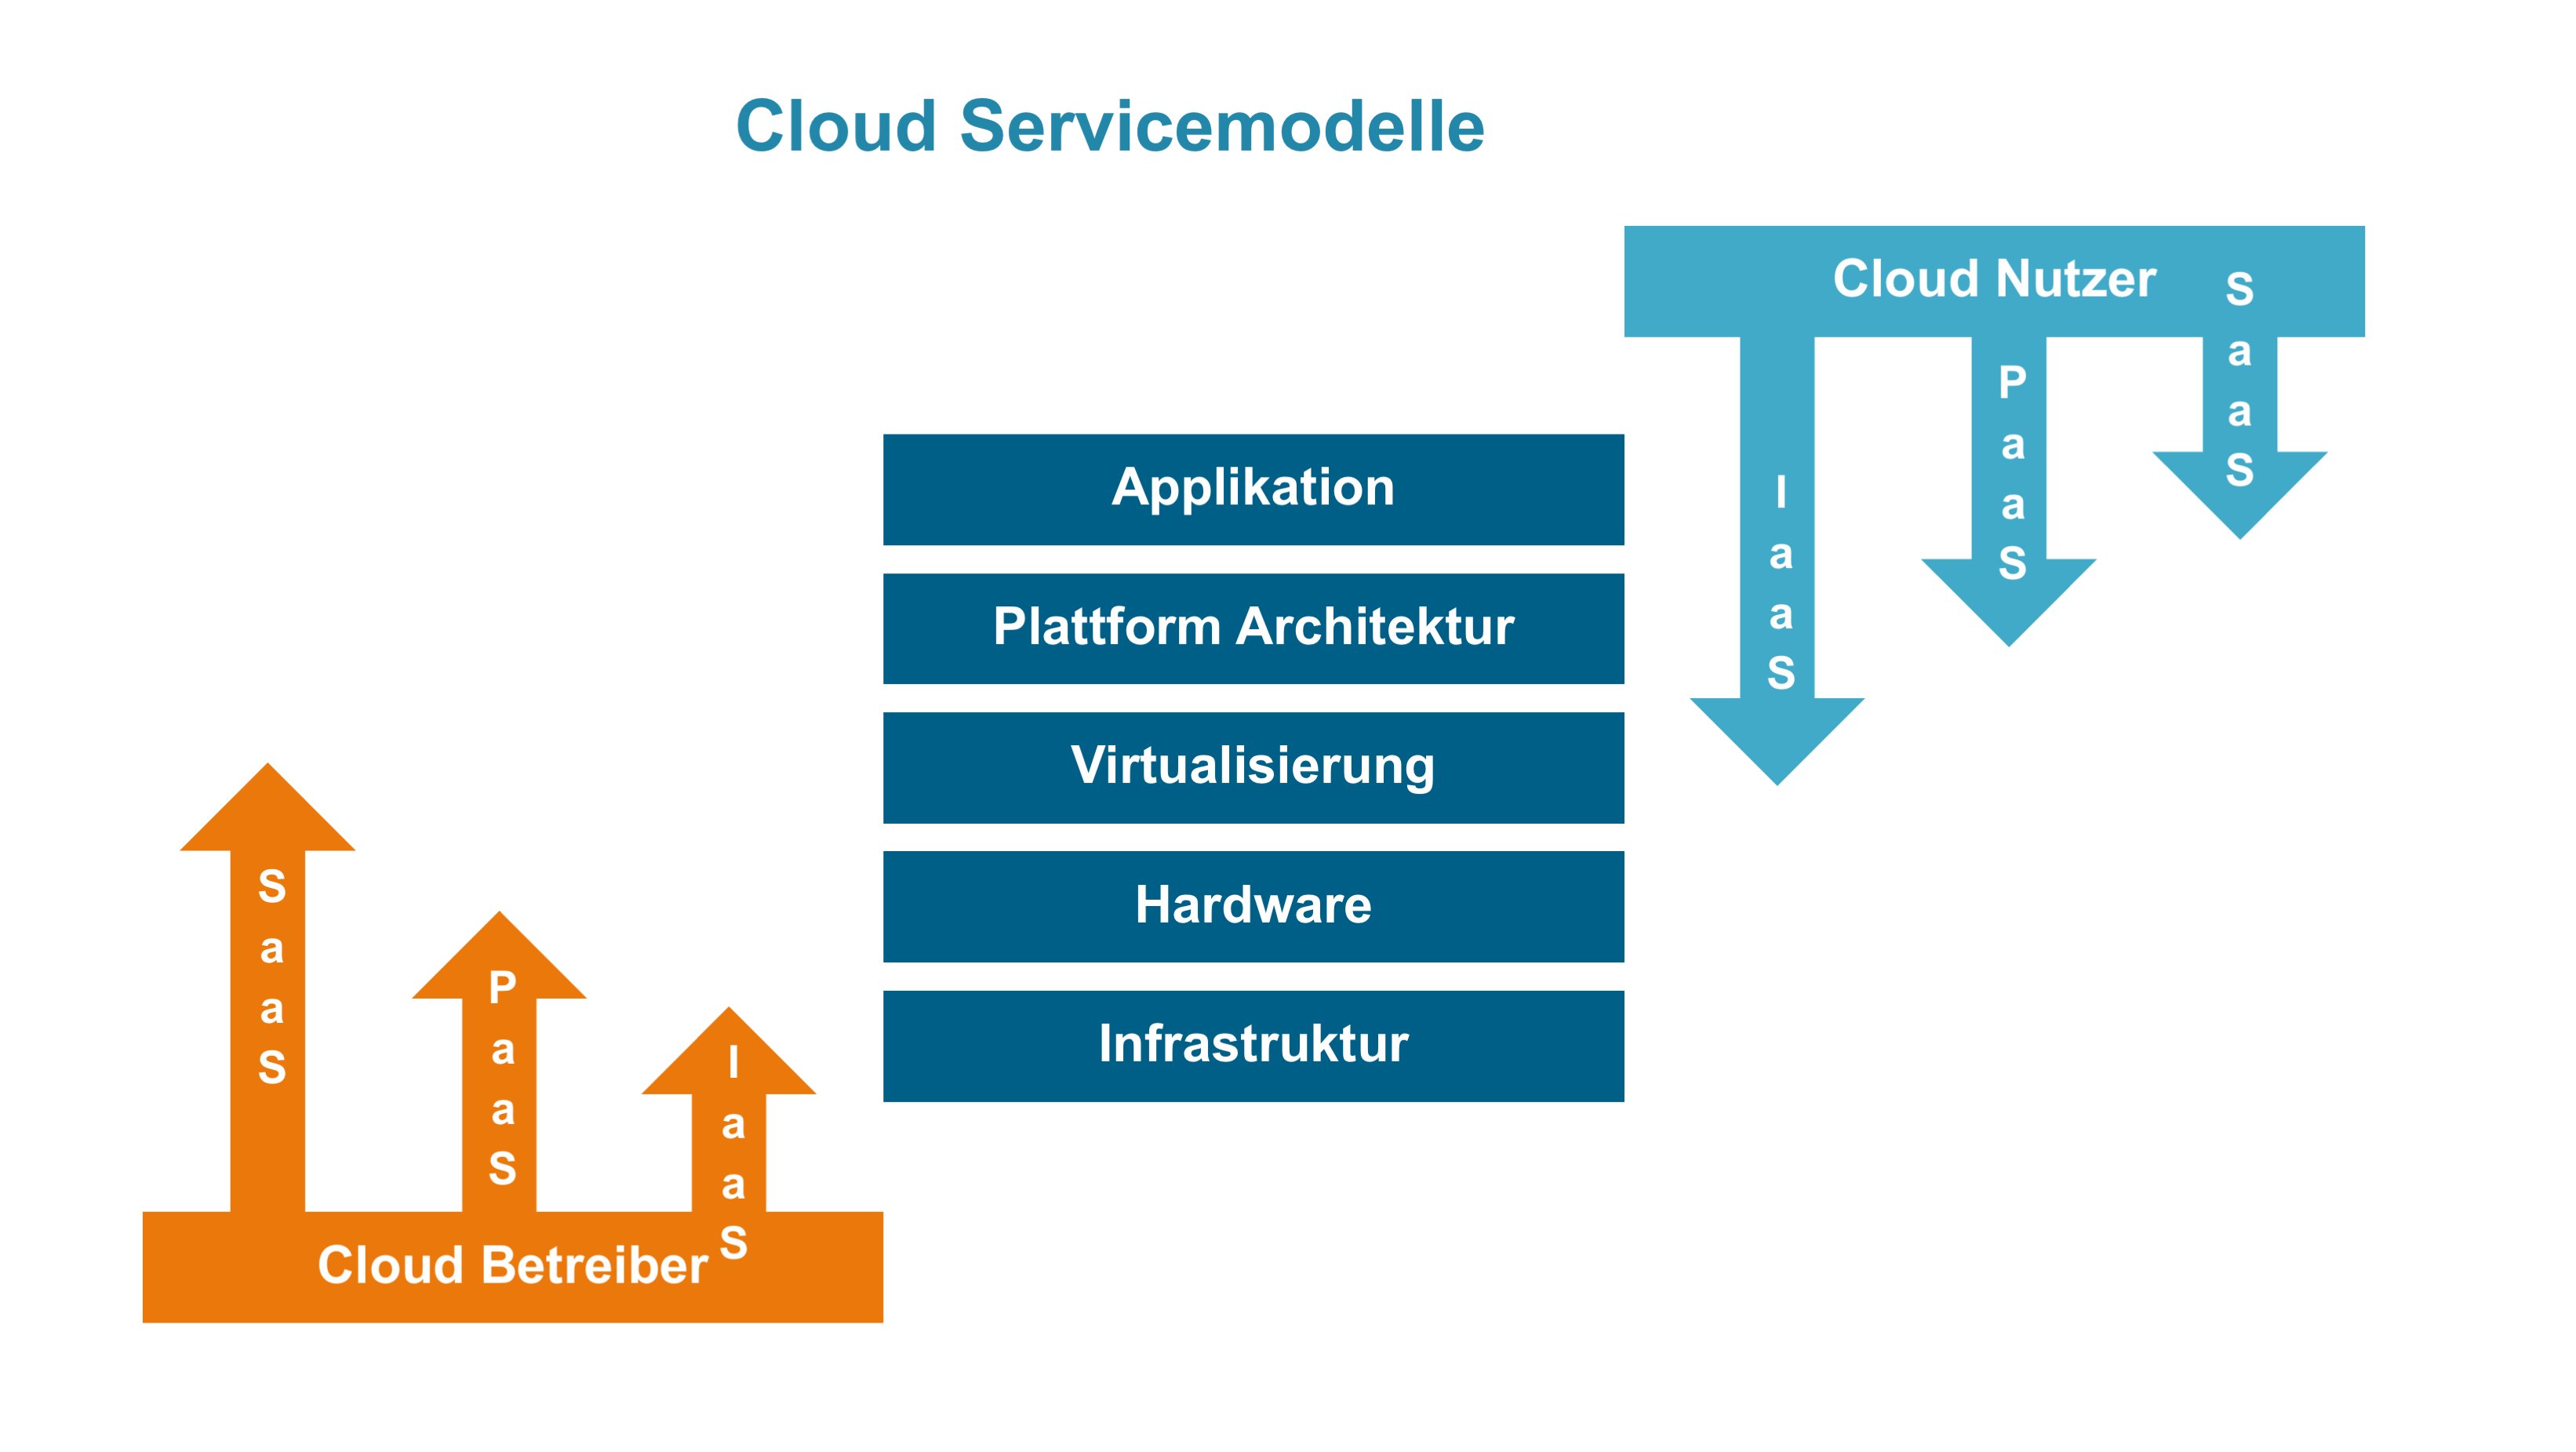
\includegraphics[width=1\textwidth]{CloudServiceModelle.png} 
\caption{Unterschiede in Zugriff und Kontrolle bei Cloud Servicemodellen (vgl. \cite{gilchrist2016industry}).}
\label{fig:cloud}
\end{figure}

\section{Begriffsabgrenzung "`Internet of Things"'}
Im Bereich von \textit{\ac{IoT}} oder Internet der Dinge werden die Begriffe \ac{IoT}, \acl{IoE}, \acl{IIoT} und Internet 4.0 beinahe gleichbedeutend verwendet \parencite{gilchrist2016industry, stackowiak2015big}. Während General Electric den Terminus "`Industrielles Internet"' prägte, entstand im Umfeld von Cisco der Begriff "`\ac{IoE}"'. Der US-amerikanische Wissenschafter Kevin Ashton verwendete 1999 zum ersten Mal den Begriff \ac{IoT} \parencite{ashton2011internet}. 

\subsection{Internet of Things}
\ac{IoT} bezeichnet jene allgegenwärtigen Dinge oder Objekte (z.B. \acl{RFID} Tags, Sensoren), welche mit ihren Nachbarn interagieren, kommunizieren und kooperieren, um gemeinsame Ziele zu erreichen \parencite{batallabeyond}. Die Kommunikation erfolgt dabei mit Hilfe des Internets. Zusätzlich werden diese Vorgänge mit einem Minimum an menschlicher Intervention durchgeführt. Die Trennung zwischen physischer und virtueller Welt verschwindet dabei \parencite{vogel2017handbuch}. 

\ac{IoT} besteht aus physischen Objekten unterschiedlichster Art (z.B. Anlagen, Maschinen oder Sensoren). Dabei benötigen alle Teilnehmer eine eindeutige Identifizierung.  

Bereits in den 1970er-Jahren gab es erste Versuche, ein Netzwerk innerhalb von "`Dingen"' aufzubauen \parencite{jeschke2017industrial}. Ein Sammelbegriff dafür ist \ac{CIM}. Diese Technologie stieß jedoch noch auf Grenzen. Diese lagen darin, dass die \acl{IKT} noch unausgereift war, Computer eine noch zu geringe Rechenleistung hatten und zu kleine Datenspeicher zur Verfügung standen. Darüber hinaus waren die Übertragungsraten zu klein und Software Tools und Formate für den Datenaustausch fehlten.

Mittlerweile haben sich die technischen Möglichkeiten in vielen Bereichen stark verbessert. Zum Beispiel haben sich in der Sensortechnologie die Größe und die Kosten der einzelnen Sensoren in den letzten Jahren massiv reduziert sowie die Verlässlichkeit verbessert, sodass immer mehr Betriebe auf diese Technologie vertrauen. Das Miniaturisieren der Sensoren ist soweit vorangeschritten, dass es aktuell Sensoren mit der Größe von Sandkörnern gibt \parencite{gilchrist2016industry}.

Von Siemens AG, Digital Factory, wurden 2017 folgende Zahlen bzgl. Siemensprodukte bekannt gegeben: 30 Millionen Automatisierungssysteme, 70 Millionen Smart Meters und 800.000 verbundene Produkte sind derzeit aktiv.

Laut einer Studie der Siemens AG werden derzeit rund 5,5 Millionen "`Dinge"' pro Tag neu vernetzt. Eine Prognose von Siemens AG schätzt, dass sich die Anzahl der verbundenen Assets im Zeitraum von 2017 bis 2020 annähernd verdoppeln  und ca. 50 Milliarden umfassen wird (siehe Abb.~\ref{fig:NumberOfAssets}).

\begin{figure}%[H]
\centering
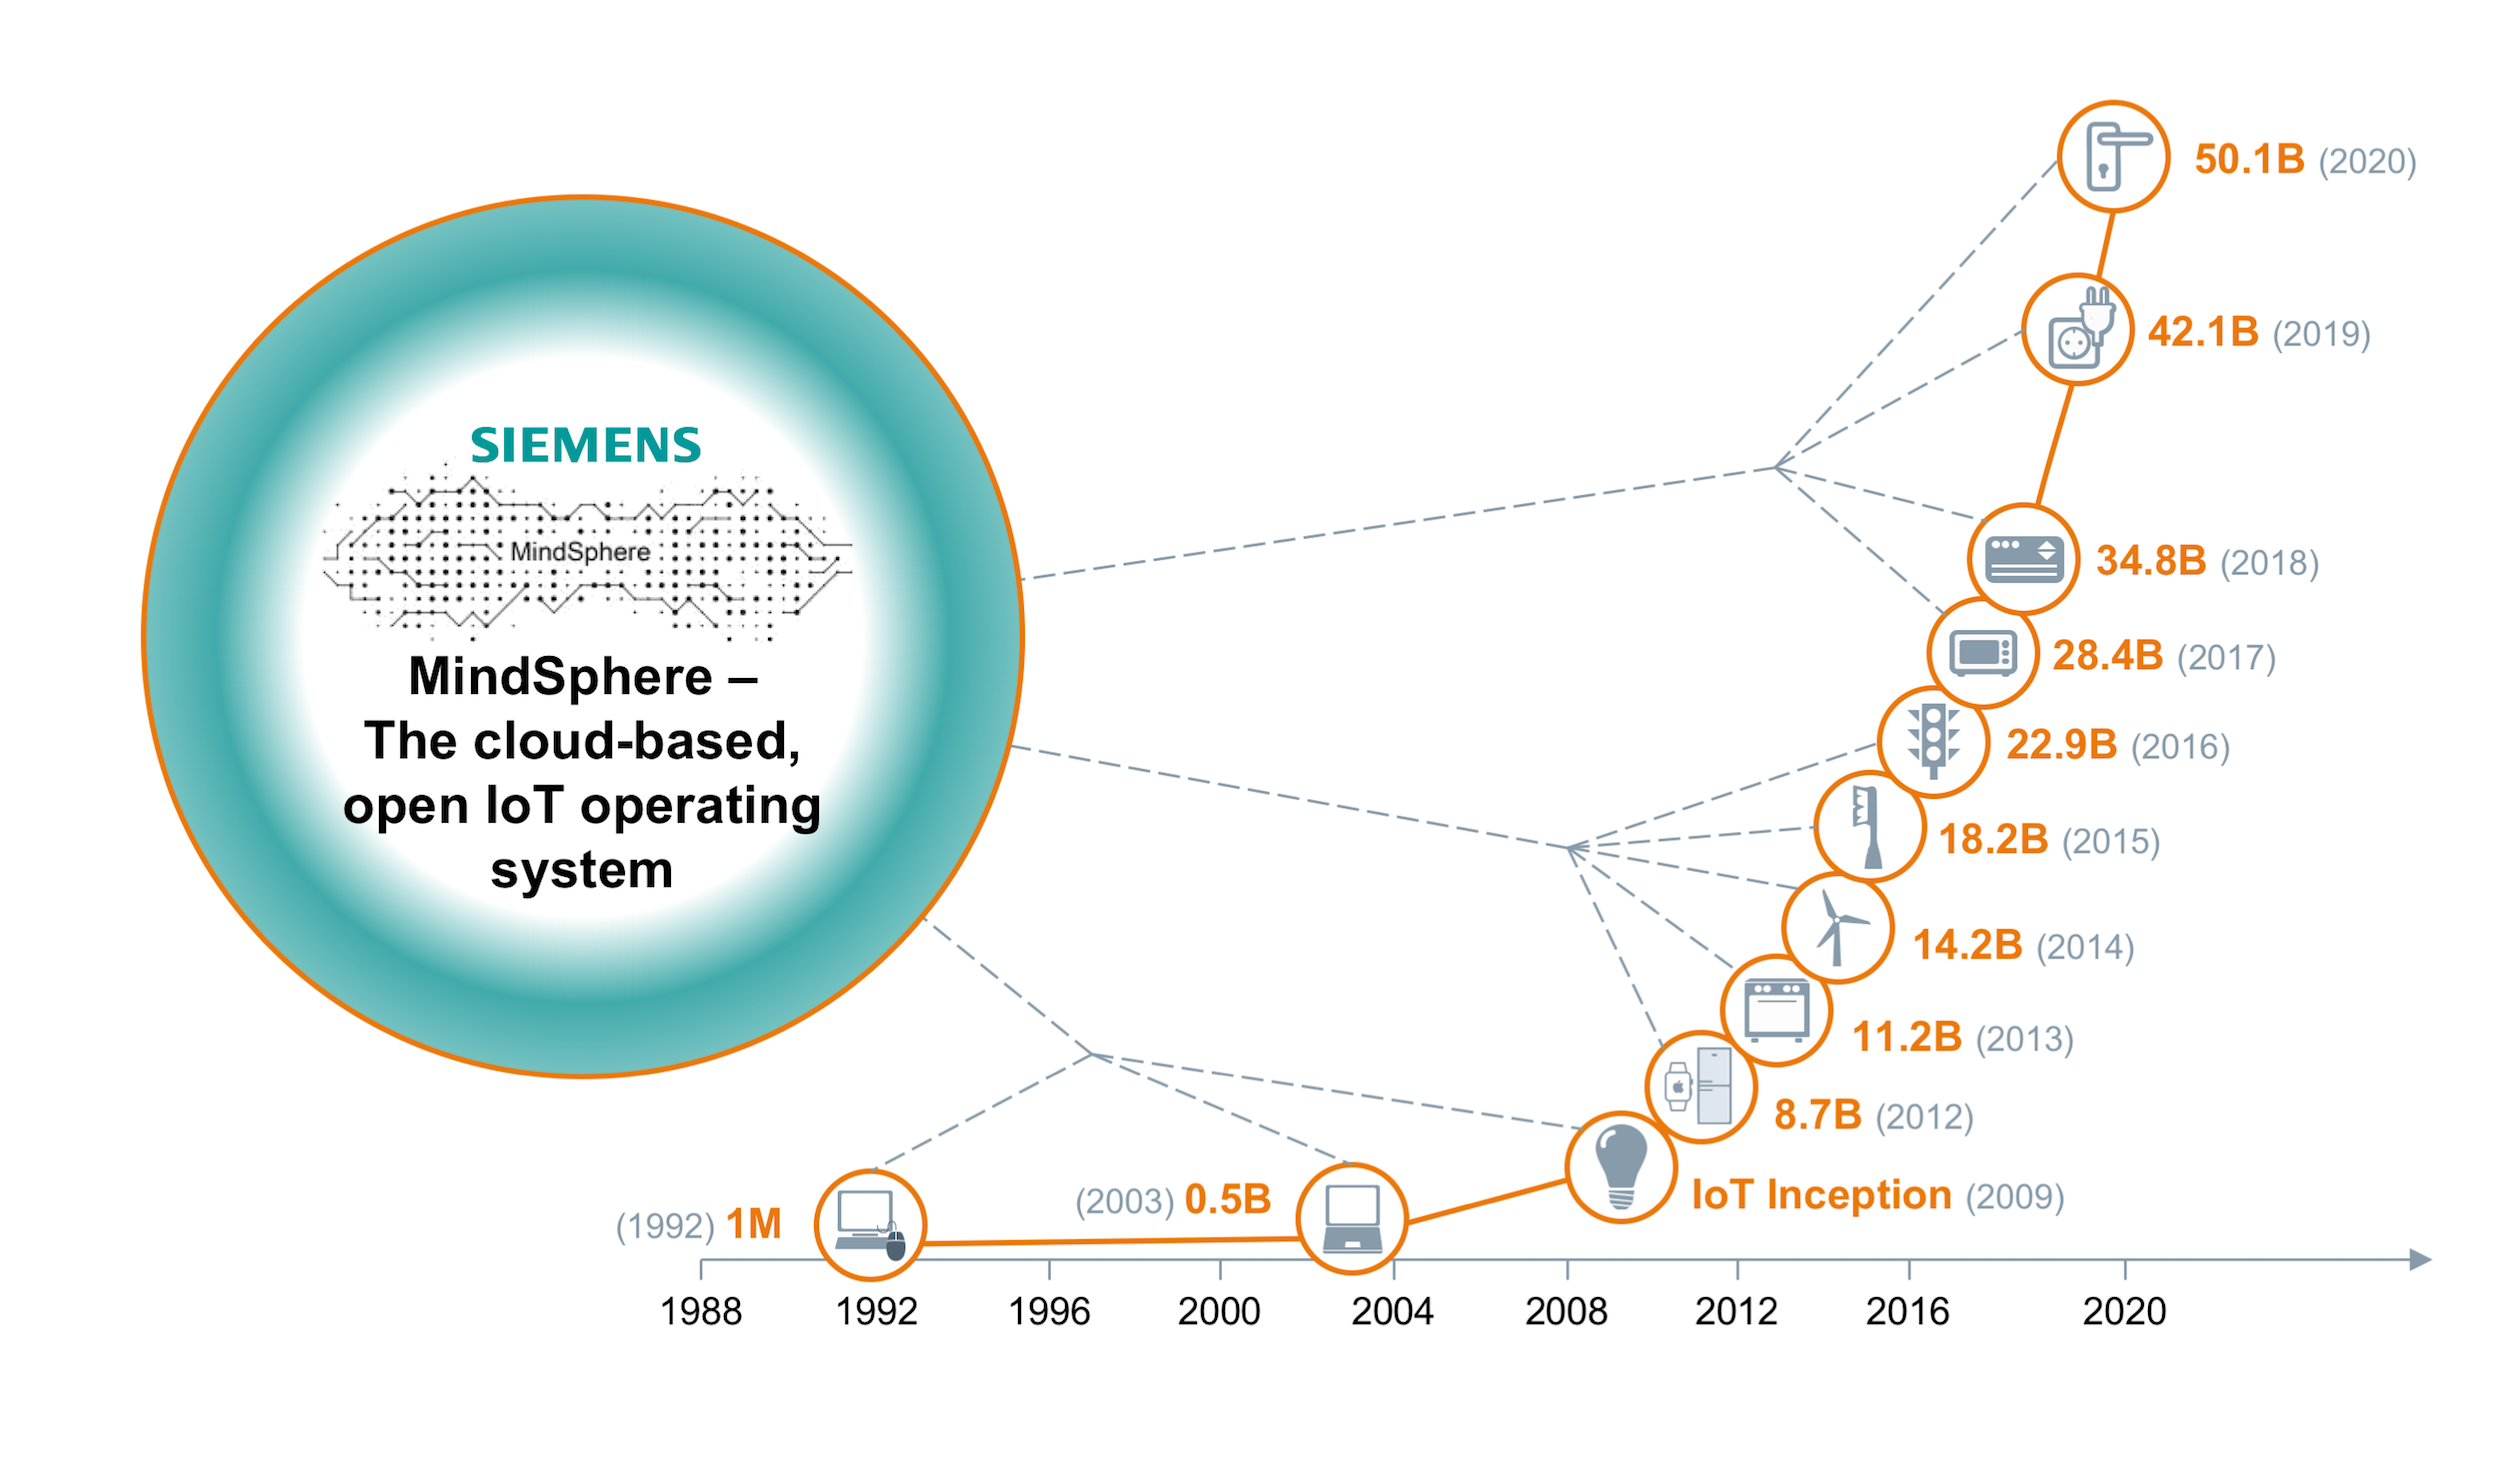
\includegraphics[width=1\textwidth]{NumberOfAssets_2.png} 
\caption{Darstellung des prognostizierten Anstiegs der Anzahl der verbundenen Assets \cite{SiemensMSIntroduction}.}
\label{fig:NumberOfAssets}
\end{figure}

\subsection{Internet of Everything}
Im Unterschied zu \ac{IoT} beschränkt sich \ac{IoE} nicht nur auf die Dinge, welche über das Internet verbunden werden, sondern bezieht auch den Menschen direkt mit ein. Die Interaktion Mensch-Gerät soll dadurch vereinfacht und erleichtert werden \parencite{andelfinger2014internet}. 

\ac{IoE} kann also auch als Netzwerk, welches Menschen, Dinge, Prozesse und Daten verbindet, bezeichnet werden; Verbindungen werden automatisiert und Menschen selbst zu "`Internetknoten"' \parencite{batallabeyond}. Ziel ist es, schnelle persönliche Kommunikation zu ermöglichen und neue Information sichtbar zu machen.

Bisher verbinden sich Menschen aktiv mit Hilfe verschiedener Geräte mit dem Internet. Durch \ac{IoE} verbinden sich unterschiedlichste Geräte im Umkreis von Personen selbständig mit dem Internet \parencite{batallabeyond}.
 
"`Wearables"' stellen einen speziellen Bereich von \ac{IoE} dar. Dabei handelt es sich um Gegenstände, welche mit Sensoren ausgestattet sind und am oder im Körper getragen werden \parencite{andelfinger2014internet}. Dabei kann es sich zum Beispiel um intelligente Ringe oder andere Schmuckstücke handeln, welche permanent den Blutdruck oder andere Vitalfunktionen ihres Trägers messen. 

Ein weiterer Einsatz von Wearables im medizinischen Bereich sind zum Beispiel Tabletten mit integrierten Sensoren \parencite{batallabeyond}. Falls es sich dabei um lebenserhaltende Medikamente handelt, wird über die Sensoren festgestellt, ob die Einnahme zeitgerecht erfolgt ist. Ist die Einnahme nicht erfolgt, wird eine automatische Alarmierung und in Folge eine Rettungskette direkt über die Datenübertragung der Sensoren eingeleitet \parencite{batallabeyond}. Ansonsten senden die Sensoren diverse Messdaten direkt vom Verdauungstrakt an den behandelten Arzt.

Weitere Beispiele für \ac{IoE} findet man in den Bereichen Smart Home und Home Automation, Smart Grid und \acl{AR}.

\subsection{Industrial Internet of Things}
Im industriellen Umfeld wird die Anwendung von \acl{IoT} oft als \ac{IIoT} bezeichnet, welches Thema des 46. World Economic Forum 2016 in Davos war.

Industrielles Internet steht noch immer am Beginn seiner Entwicklung. Sensoren und Geräte (Devices), welche Daten zur Kontrolle von Operationen liefern, gibt es schon seit vielen Jahren. Außerdem gibt es schon lange \ac{M2M} Kommunikation. Also ist der Kern von \ac{IIoT} eigentlich nichts Neues \parencite{gilchrist2016industry}. Wie in Abbildung~\ref{fig:M2MIIoT} erkennbar, unterscheiden sich die Architekturen von \ac{M2M} und \ac{IIoT} lediglich durch das Einbinden der Cloud-Komponente \parencite{gilchrist2016industry}.

\begin{figure}%[H]
\centering
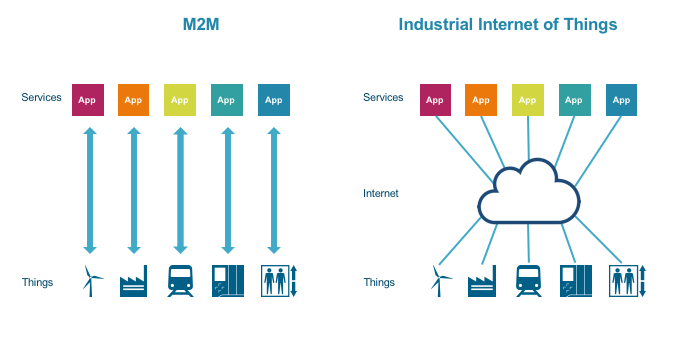
\includegraphics[width=1\textwidth]{M2M_IIoT.png} 
\caption{Gegenüberstellung Architekturen \ac{M2M} und \ac{IIoT} (vgl.\cite{gilchrist2016industry}).}
\label{fig:M2MIIoT}
\end{figure}

Der Hauptnutzen von \ac{IIoT} ist eine bessere Sichtbarkeit und mehr Einblick in die Operationen eines Betriebes \parencite{gilchrist2016industry}. Weitere Ziele liegen darin, erhöhte Profite zu erzielen, schnellere und optimierte Prozesse zu erhalten, die Ausgaben zu reduzieren und die Gesundheit und Sicherheit der Mitarbeiter in der Produktion zu steigern. 

Gegenüber einfacher \ac{M2M} Kommunikation ist die Skalierung von \ac{IIoT} eine andere: Daten können hier mit Hilfe von IIoT-Systemen in Cloud Systemen gesammelt, gespeichert, analysiert und zurück zum Gerät als Kontroll-Feedback geschickt werden. 

Dabei wird die gesamte Produktionskette vernetzt; Maschinen können miteinander kommunizieren und einzelne Produktionsschritte selbstständig steuern \parencite{andelfinger2014internet, gilchrist2016industry}. Voraussetzung dafür ist, dass sämtliche Maschinen bzw. Anlagenteile mit Sensoren ausgestattet werden. In der Folge werden präzise Daten zum Status der Maschinen sowie zu den erzeugten Produkten geliefert. Optimierungen der Produktionsabläufe sowie eine möglichst einfache und kostenschonende Wartung sind dabei das Ziel. Erst dadurch wird eine vorausschauende Arbeit und teilweise auch Selbstdiagnose der Maschinen möglich.

Die Steuerung der Produktionsprozesse in intelligenten Fabriken (Smart Factories) oder auch digitalen Fabriken (Digital Factories) (siehe Abb.~\ref{fig:smartFactory}) erfolgt automatisiert und Eingriffe von außen werden minimiert.

\begin{figure}%[H]
\centering
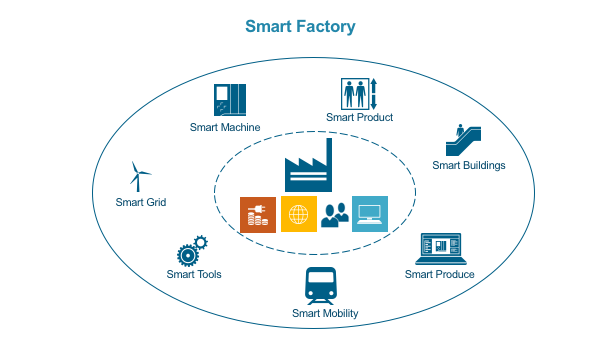
\includegraphics[width=1\textwidth]{SmartFactory.png} 
\caption{Struktur Smart Factory (vgl.\cite{gilchrist2016industry}).}
\label{fig:smartFactory}
\end{figure}

Die Vernetzung der Maschinen geht über einzelne Fabriken hinaus und vernetzt ebenso Partnerfabriken und Lieferanten bis hin zum Kunden \parencite{andelfinger2014internet}. Die Rolle des Menschen reduziert sich hier auf die Überwachung und die Entwicklung von Produktionsprozessen.

\paragraph{Einige Anwendungsgebiete von industriellem Internet (nach Gilchrist \parencite{gilchrist2016industry}):}
\begin{itemize}
\item Logistik
\item Transport
\item Luftfahrt
\item Gesundheit
\item Energieproduktion
\item Öl- und Gasförderung
\item Smart Office
\item Smart Homes - Gebäudeautomation
\end{itemize}
\vspace{\baselineskip}


\section{Siemens MindSphere}
Die Firma Siemens AG bietet seit Juli 2016 mit MindSphere\footnote{MindSphere: https://www.siemens.com/global/de/home/produkte/software/mindsphere.html} ein cloud-basiertes, offenes \ac{IoT}-Betriebssystem auf der Basis von \ac{PaaS} für digitale Services an \parencite{SiemensMSIntroduction,SiemensWhitepaper}. Industrielle Anlagen können so auf einfache Weise Daten in eine Cloud-Umgebung liefern und auch wieder abgreifen. 

\subsection{Motivation für MindSphere}

Daten von zahlreichen, bereits installierten Geräten und Maschinen werden gesammelt und in definierten Intervallen in eine Cloud übertragen. Von dort können diese Daten jederzeit wieder abgerufen bzw. ausgewertet werden. Hauptmotivation ist die Performance bzw. Leistung von sogenannten Assets\footnote{Asset bedeutet im Umfeld von MindSphere eine digitale und logische Repräsentation einer physischen Maschine oder eines Anlagenteils.} zu steigern. Mehrere ähnliche oder sogar gleiche Anlagen oder Arbeitsabläufe können somit direkt verglichen und in der Folge sowohl in Bezug auf Kosten als auch auf Herstellungszeit des Produkts optimiert werden.

Ein weiterer Aspekt ist die vorausschauende und vorbeugende Wartung -- \ac{PPM}.  Unter \ac{PPM} versteht man, dass auf Grund von stark abweichenden Daten ein Ausfall eines Anlagenteils möglichst früh und mit hoher Wahrscheinlichkeit vorausgesagt werden kann und dadurch der Wartungsaufwand und die eventuelle Ausfallszeit einer Anlage minimiert werden können. 

Mit der Datenanalyse kann auch eine Qualitätsanalyse und in der Folge eine Qualitätssteigerung der Produkte durchgeführt werden. Auch für das Garantiemanagement sind die Daten von großem Nutzen. 

Zusammenfassend sind die Ziele eine Senkung der Produktions- und Wartungskosten sowie eine Steigerung der Anlagenleistung und User Experience. Als User Experience werden die Wahrnehmungen und Reaktionen einer Person aufgrund der Nutzung eines Produkts, eines Systems oder einer Dienstleistung bezeichnet \parencite{dis20099241, hartson2012ux}.

\subsection{Aufbau MindSphere }
MindSphere ist aus drei Schichten aufgebaut (siehe Abb.~\ref{fig:MSArchitecture}) \parencite{SiemensMSIntroduction,SiemensWhitepaper}. In der untersten Schicht (Ebene 1 -- Konnektivität) erfolgt der direkte Zugang zu den physischen Geräten, in der mittleren Schicht (Ebene 2 -- Plattform) befindet sich die Cloud-Infrastruktur und in der obersten Schicht (Ebene 3 -- Applikationen) befinden sich die Applikationen.

\begin{figure}[H]
\centering
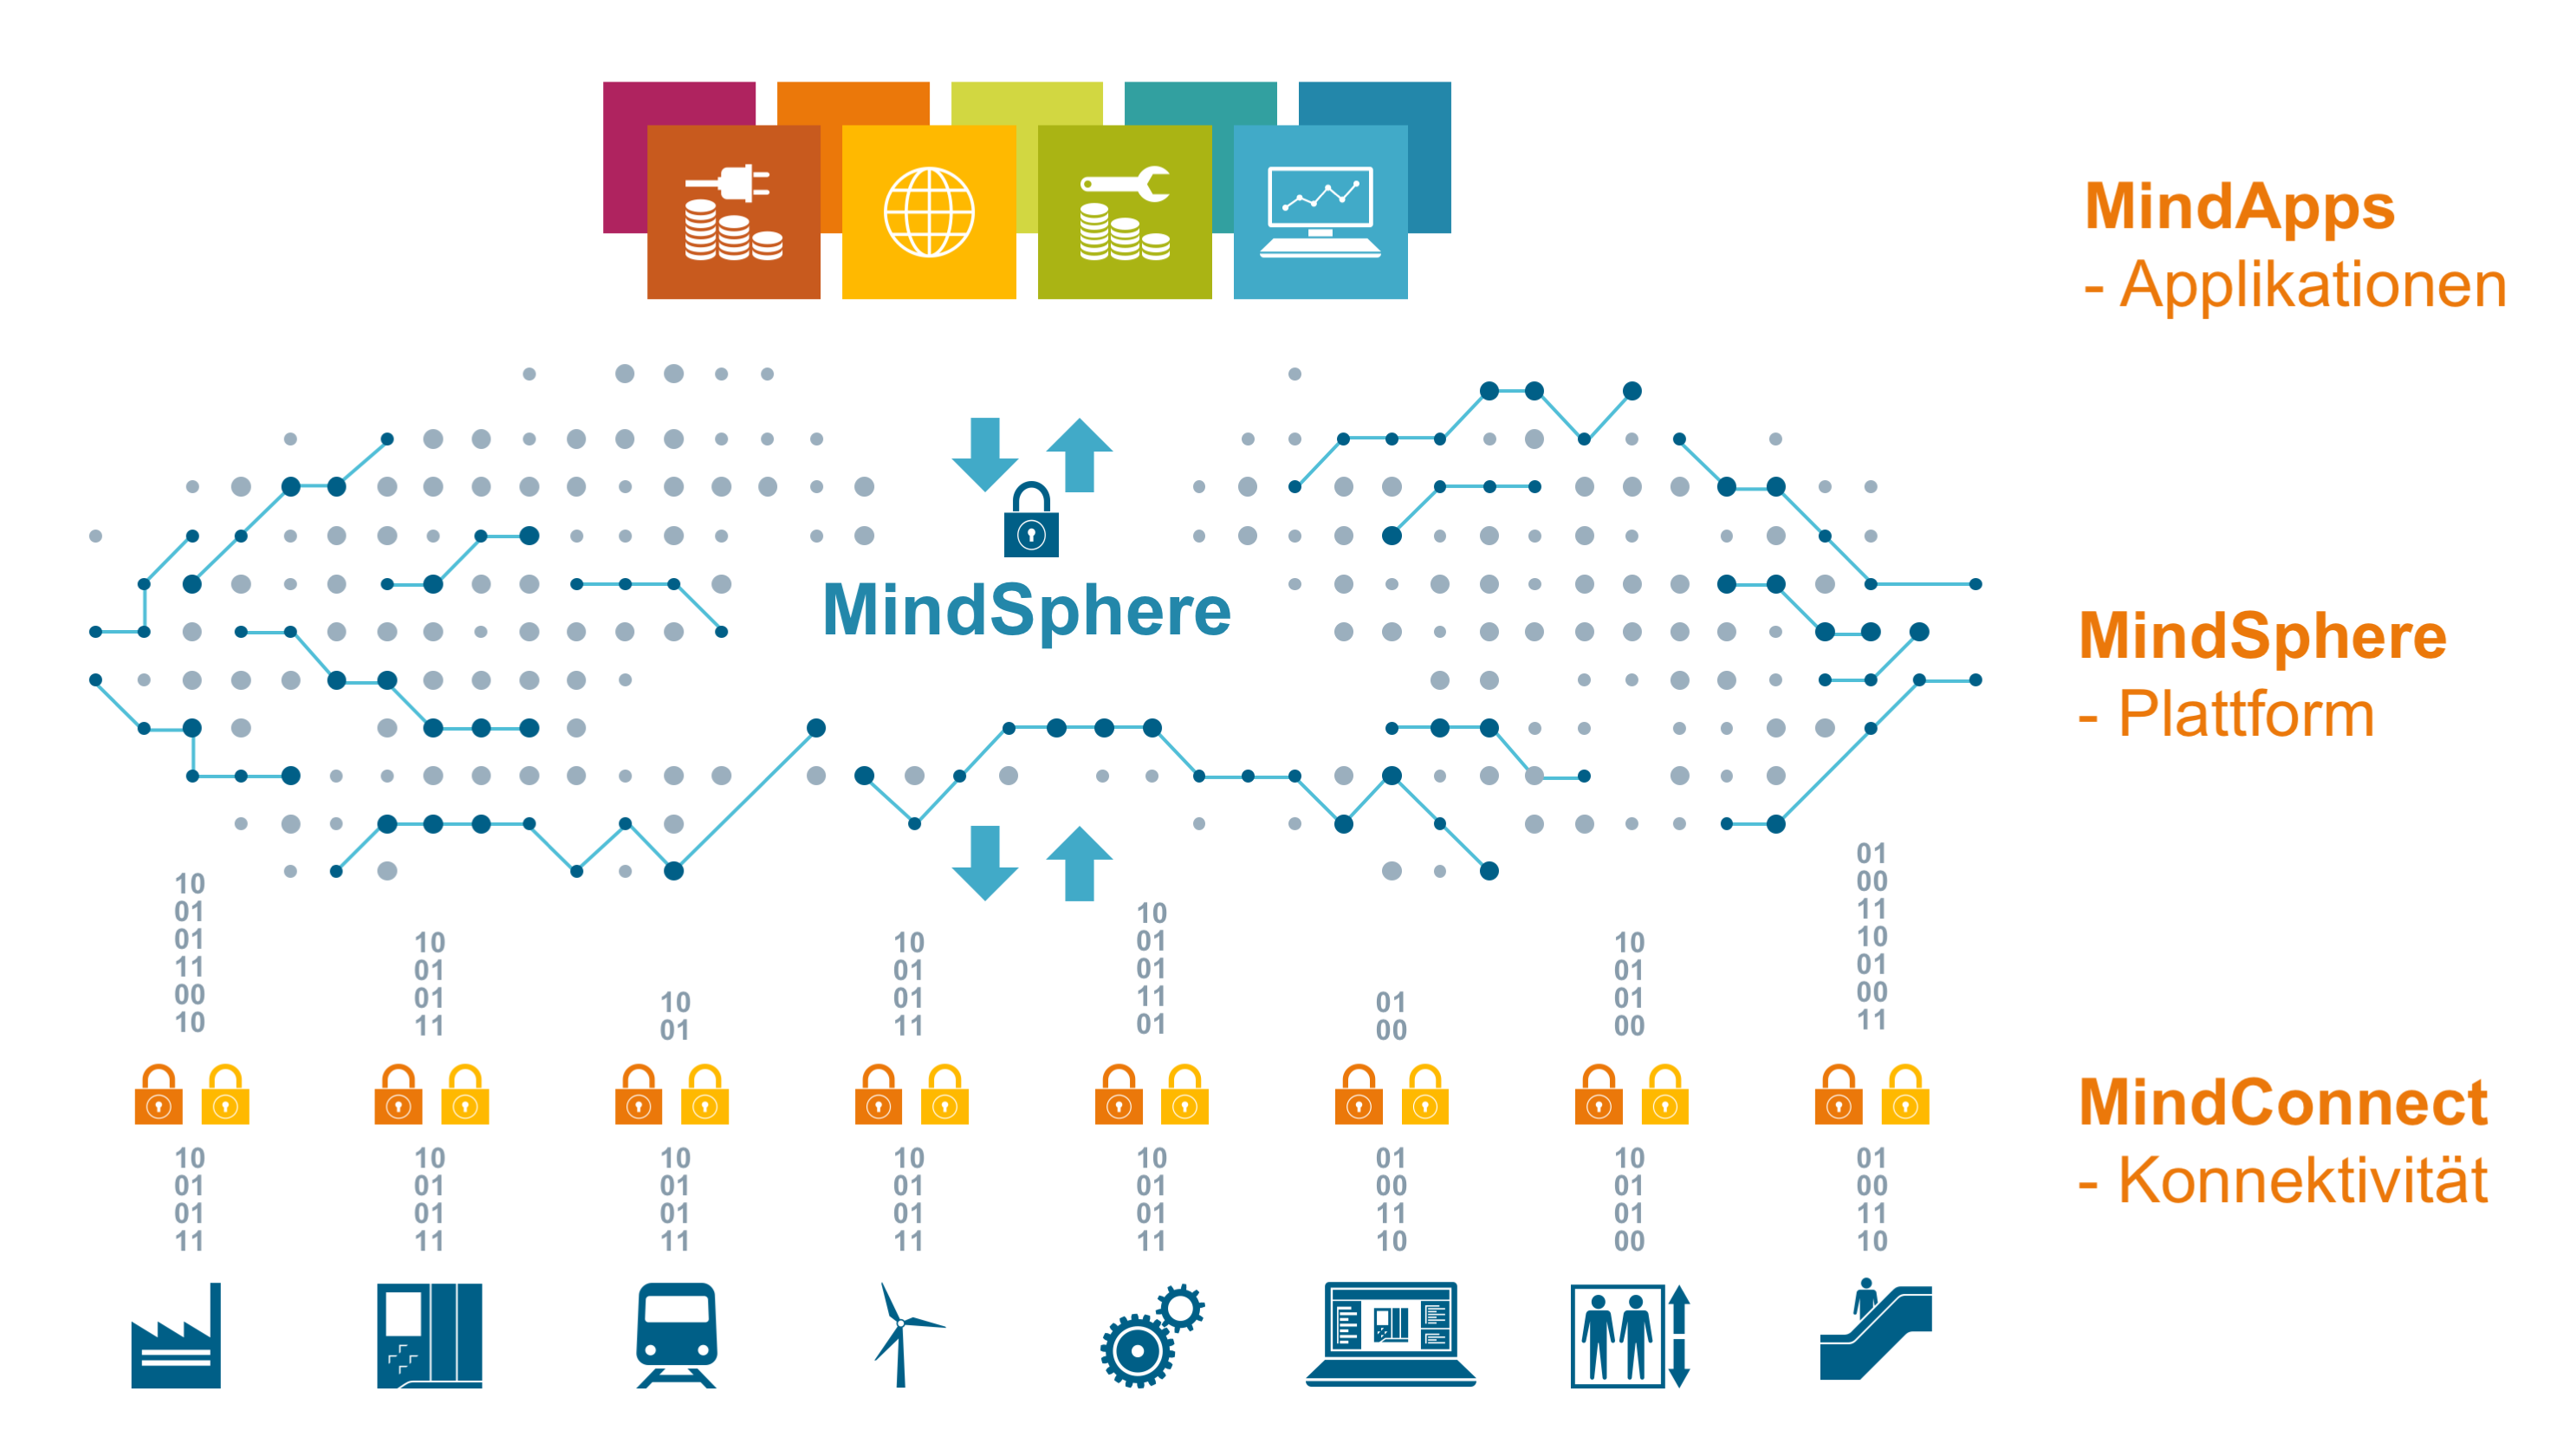
\includegraphics[width=1\textwidth]{MSArchitektur_1.png} 
\caption{Aufbau von MindSphere in drei Ebenen \cite{SiemensMSIntroduction}.}
\label{fig:MSArchitecture}
\end{figure}

\subsubsection{MindConnect}
Auf Ebene 1 -- Konnektivität -- wird durch \textit{MindConnect} eine Schnittstelle zwischen einer speicherprogrammierbaren Steuerung (\acs{SPS}) und der MindSphere Cloud hergestellt. 

Die Kommunikation zwischen den Assets und den MindConnect-Modulen erfolgt derzeit\footnote{Stand November 2017} mittels Open Standard Kommunikation wie z.B. OPC UA (Open Platform Communications Unified Architecture) oder Siemens S7 300/400 Protokoll. Für die nächste Version ist auch eine Unterstützung von z.B. MODBUS geplant. 

MindConnect bezeichnet ein physisches Gerät, welches vor Ort direkt in der Betriebsanlage an die \acs{SPS} montiert und durch Plug-and-Play verbunden wird. Hier bietet die Firma Siemens zwei Hardware-Komponenten an (siehe Abb.~\ref{fig:MSConnect}):
\vspace{\baselineskip}

\begin{figure}[H]
\centering\small
\setlength{\tabcolsep}{0mm}
\begin{tabular}{c@{\hspace{12mm}}c}
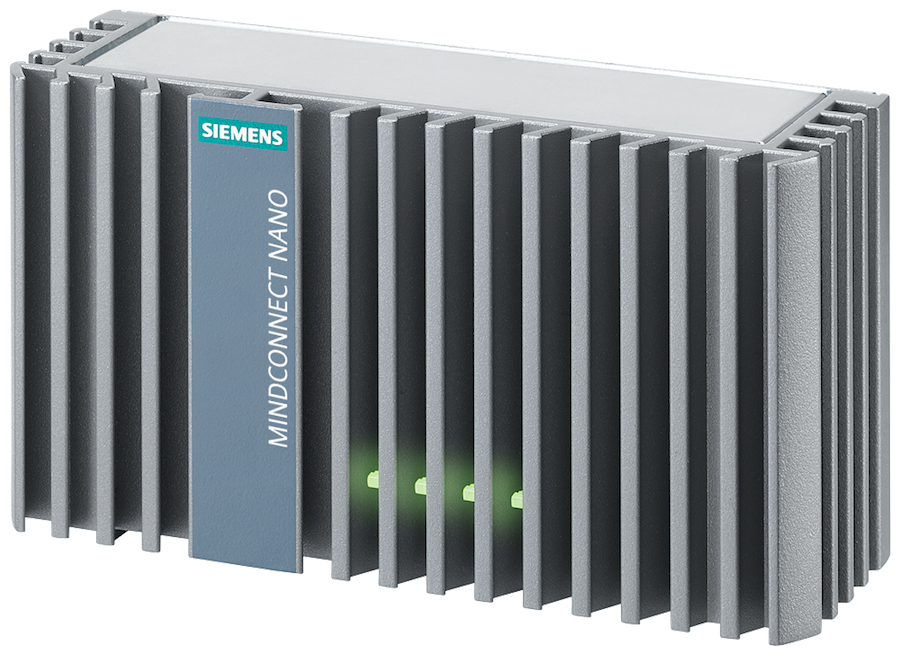
\includegraphics[width=0.45\textwidth]{MindConnect_Nano.png}&
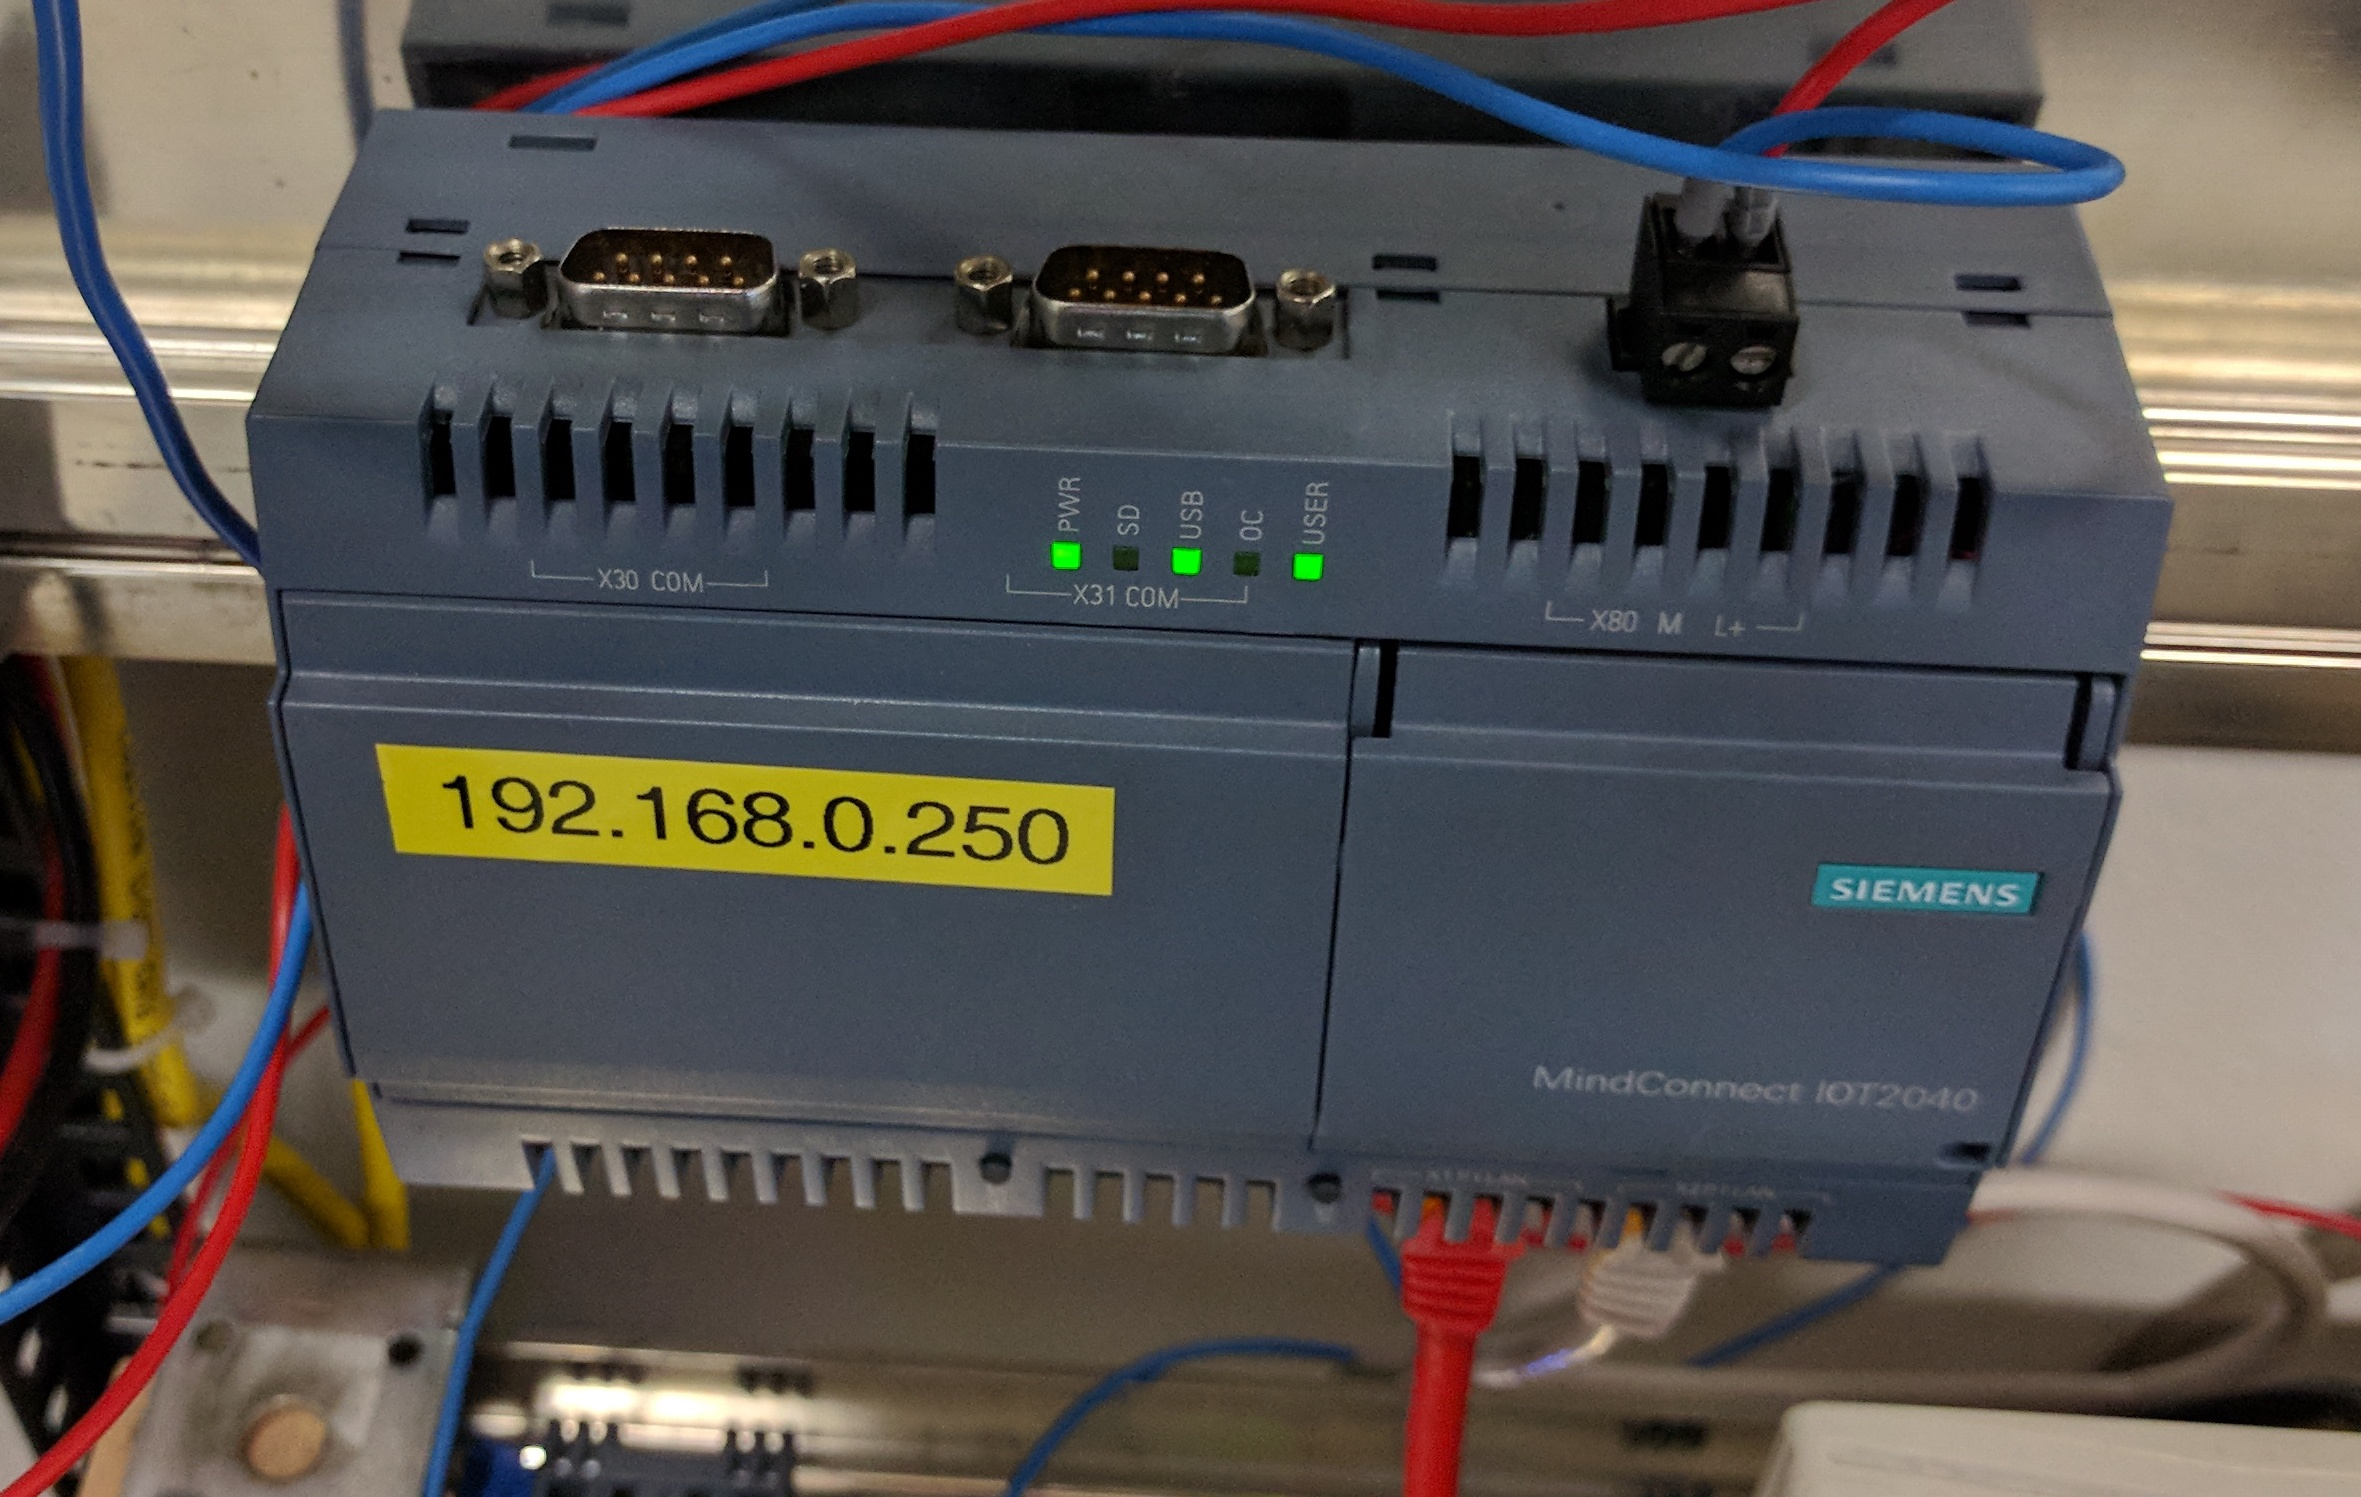
\includegraphics[width=0.45\textwidth]{MCIoT2040Foto.jpg}
\\
MindConnect Nano & MindConnect IoT2040
\end{tabular}
\caption{Siemens MindConnect Elemente \cite{SiemensMSIntroduction}.}
\label{fig:MSConnect}
\end{figure}
\vspace{\baselineskip}

\begin{itemize}
\item \ac{MCN}:\\
\ac{MCN} ist ein vorkonfigurierter Industrie-PC mit Verbindung zu MindSphere. Das Gerät unterstützt zur Datensammlung verschiedene Protokolle -- wie z.B. (OPC UA und S7 300/400). Die Datenübertragung erfolgt verschlüsselt und über eine sichere Internetverbindung. \ac{MCN} ist ausschließlich in Verbindung mit Siemens-Geräten verwendbar.

\item \ac{IoT2040}:\\
\ac{IoT2040} ist die kostengünstigere Alternative zu \ac{MCN}. Im Vergleich zu \ac{MCN} ist das \ac{IoT2040} kompakter und eher für kleinere Anlagen geeignet. Es unterstützt dieselben Protokolle wie \ac{MCN} und ist ebenfalls ausschließlich in Verbindung mit Siemens-Geräten verwendbar.
\end{itemize}
\vspace{\baselineskip}

Zusätzlich zu den physischen Geräten gibt es noch zwei weitere Möglichkeiten, Daten in die MindSphere Cloud zu laden:
\vspace{\baselineskip}

\begin{itemize}
\item MindConnect FB1500:\\
MindConnect FB1500 ist eine Siemens Totally Integrated Automation (TIA) Portal STEP7 Bibliothek, um die Funktionalität der Siemens S7-1500 \acs{SPS} zu erweitern. Diese Bibliothek unterstützt die verschlüsselte Übertragung von \acs{SPS}-Daten in die MindSphere Cloud. Die Konfiguration des Datenmodells erfolgt in STEP7 (TIA Portal V14). Zusätzliche Hardware ist nicht erforderlich.

\item MindConnect LIB:\\
MindConnect LIB ist ein Software Entwicklungssystem, welches die Programmierung gegen die Schnittstellen von MindSphere erlaubt. Das Kernstück der MindConnect LIB besteht aus einer C-basierten Software-Bibliothek. MindConnect LIB ist geräteunabhängig und sowohl in Verbindung mit Siemens-Geräten als auch Geräten von Drittanbietern verwendbar.
\end{itemize}
\vspace{\baselineskip}

Eine Gegenüberstellung der einzelnen MindConnect Geräte in Bezug auf Pufferspeichergröße, unterstützte Protokolle, Lese- und Transferzyklen ist in Tabelle \ref{tab:mindConnect} ersichtlich.

\begin{table}[H]
	\caption{Gegenüberstellung der einzelnen MindConnect Geräte \cite{SiemensWhitepaper}.} 		\label{tab:mindConnect}
	\centering
	\setlength{\tabcolsep}{5mm} % separator between columns 
	\def\arraystretch{1.25} % vertical stretch factor 
	\begin{tabular}{r|ccc}
 	  % \hline
   		& \emph{MC Nano} & \emph{IoT2040} & \emph{FB1500} \\
    	\hline
    	%\hline
    	Lokaler Pufferspeicher & 500MB & 500MB & 500MB \\
    	%\hline
    	Unterstützte Protokolle & S7/OPC UA & S7/OPC UA & S7-1500 \\
    	%\hline
   	 	max. Datenlesezyklus\\(Datenpunkte/Sek.) & 250 & 30   & 110 \\
    	%\hline
        min. Datentransferzykluszeit\\(in Sek.) & 10 & 10   & 10 \\
    	%\hline
  	\end{tabular}
\end{table}

\subsubsection{MindSphere Cloud}
Auf der Ebene 2 -- Plattform -- befindet sich die \textit{MindSphere-Cloud-Infrastruktur}. Derzeit wird die Cloud-Infrastruktur von SAP Cloud Foundry\footnote{SAP Cloud Foundry: https://cloudplatform.sap.com/index.html} als offene Plattform mit \ac{PaaS} zur Verfügung gestellt. Für die Zukunft ist eine Zusammenarbeit mit weiteren großen Partnern wie Amazon Web Services\footnote{Amazon Web Services: https://aws.amazon.com/}, AtoS\footnote{AtoS: https://atos.net/de-at/austria} und Microsoft Azure\footnote{Microsoft Azure: https://azure.microsoft.com/de-de/} geplant \parencite{SiemensMSIntroduction}. 

\subsubsection{MindApps}
Darüber befindet sich auf Ebene 3 -- Applikationen -- die \textit{MindApps} -Applikationsschicht. Industrielle Applikationen werden hier entwickelt. Mit Hilfe dieser Webapplikationen können die Daten einerseits dargestellt und andererseits analytisch ausgewertet werden. 

MindApps werden auf Basis von HTML5 entwickelt und daher in einem Browser betrieben.

\subsection{Stärken von MindSphere}
Durch die Cloud-Infrastruktur basierend auf SAP Cloud Foundry wird eine gute Skalierbarkeit erreicht \parencite{SiemensMSIntroduction,SiemensWhitepaper}. Das bedeutet, dass sowohl kleine Datenmengen (wenige MB) als auch Big Data verarbeitet werden können. Im Bezug auf Datenmenge ist es möglich schnell -- auch temporär-- auf- oder abzuskalieren. 
\vspace{\baselineskip}

Weitere Vorteile:
\begin{itemize}
\item Hohe Sicherheitsstandards:
MindConnect Elemente basieren auf \ac{ICS}-Sicherheit, orientiert an Industrie Standard IEC 62443\footnote{IEC 62443: Industrial communication networks – Network and system security} und ISO 27001\footnote{ISO 27001: Information technology – Security techniques – Information security management systems – Requirements} \parencite{SiemensMSMCSecurity}. Aus Sicherheitsgründen ist es nur möglich, Daten über die MindConnect Elemente aus den Assets zu extrahieren und nicht Daten in die Assets einzuspielen. Die Datenübertragung erfolgt mit mindestens 256 Bit SSL/TLS-Verschlüsselung.
\item Hohe Anzahl an installierten Geräten:
Derzeit gibt es im Umfeld Siemens ca. 30 Millionen Automatisierungssysteme, ca. 70 Millionen Smart Meter und ca. 800.000 vernetzte Produkte, welche potentiell mit MindSphere verbunden werden können.
\item Digitalisierung:
Durch die Möglichkeit eines digitalen Zwillings lassen sich optimierte Simulation und Engineering realisieren.
\item Einfache Anbindung:
Das Plug-and-Play-System bei der Installation der MindConnect Elemente ermöglicht eine schnelle Anbindung der Assets. 
\item REST:
Die Kommunikation ist auf Grund einer HTTP-basierter RESTfull API Firewall- und Entwickler-freundlich.  
\end{itemize}

\subsection{Technische Einschränkungen}
Folgende technische Einschränkungen existieren derzeit \parencite{SiemensMSTraining}: 

\begin{itemize}
	\item \acl{MCN}:
    	\begin{itemize}
			\item Es können maximal 250 Float-Werte alle fünf Sekunden gelesen werden.
			\item Es können maximal 10 Variablen jede Sekunde gelesen werden.
			\item Maximal drei S7-\ac{SPS} können mit einem MCN verbunden werden. 
			\item Maximal acht OPC UA Server können mit einem MCN verbunden werden. 
		\end{itemize}
  	\item \ac{IoT2040}:
        \begin{itemize}
			\item Das minimale Datenübertragungs-Intervall beträgt 15 Sekunden.
			\item Es können maximal 30 Float-Werte alle 15 Sekunden gelesen werden.
			\item Maximal drei S7 können mit einem IoT2040 verbunden werden.
			\item Maximal acht OPC UA Server können mit einem IoT2040 verbunden werden.
		\end{itemize}    
  	\item FB1500:
        \begin{itemize}
			\item Es können maximal 250 Float-Werte pro Sekunde gelesen werden.
			\item Es können maximal 10 Variablen jede Sekunde gelesen werden.
			\item Die Konfiguration kann nur per TIA Portal geändert werden.
		\end{itemize}
     \item Konfigurations- bzw. Kommissionierungs-Restriktionen:
         \begin{itemize}
			\item Nach dem Anlegen können Aspects deaktiviert jedoch nicht gelöscht werden.
			\item Es sind nur maximal 200 Endkunden pro Mieter möglich.
		\end{itemize}
\end{itemize}

\subsection{Überblick über das MindSphere-Preismodell}
Siemens AG verwendet ein Pay-per-use-Preismodell. Bei der Verwendung von MindSphere fallen Kosten in folgenden Bereichen an (siehe Abb.~\ref{fig:PriceModel}):

\begin{itemize}
	\item Investition MindConnect:\\
    Für die Hardwarekomponenten \ac{MCN} und \ac{IoT2040} ist pro Gerät eine einmalige Gebühr zu entrichten. Bei den MindSphere-Varianten mit FB1500 und MindConnect LIB fallen keine Investitionsgebühren an.    	
  	\item Monatsgebühr MindAccess:\\
    Um Daten in die MindSphere Cloud speichern bzw. Daten wieder abgreifen zu können, ist eine Berechtigung mittels Zugangskonto erforderlich. Bei diesen Zungangskontos gibt es zwei Arten -- Benutzer- und Entwicklerkonto. Je nach Kontoart und den damit verbundenen Berechtigungen fallen monatliche Gebühren an.
  	\item Monatsgebühr Datenmodell:\\
    Die monatliche Gebühr für die Datenübertragung und Datenspeicherung wird für jeden Kunden nach dem jeweiligen Bedarf abhängig von der Anzahl der Datenpunkte, dem Datentyp der Messdaten, dem Lesezyklus und der Anzahl der Assets berechnet. 
\end{itemize}

\begin{figure}[H]
\centering
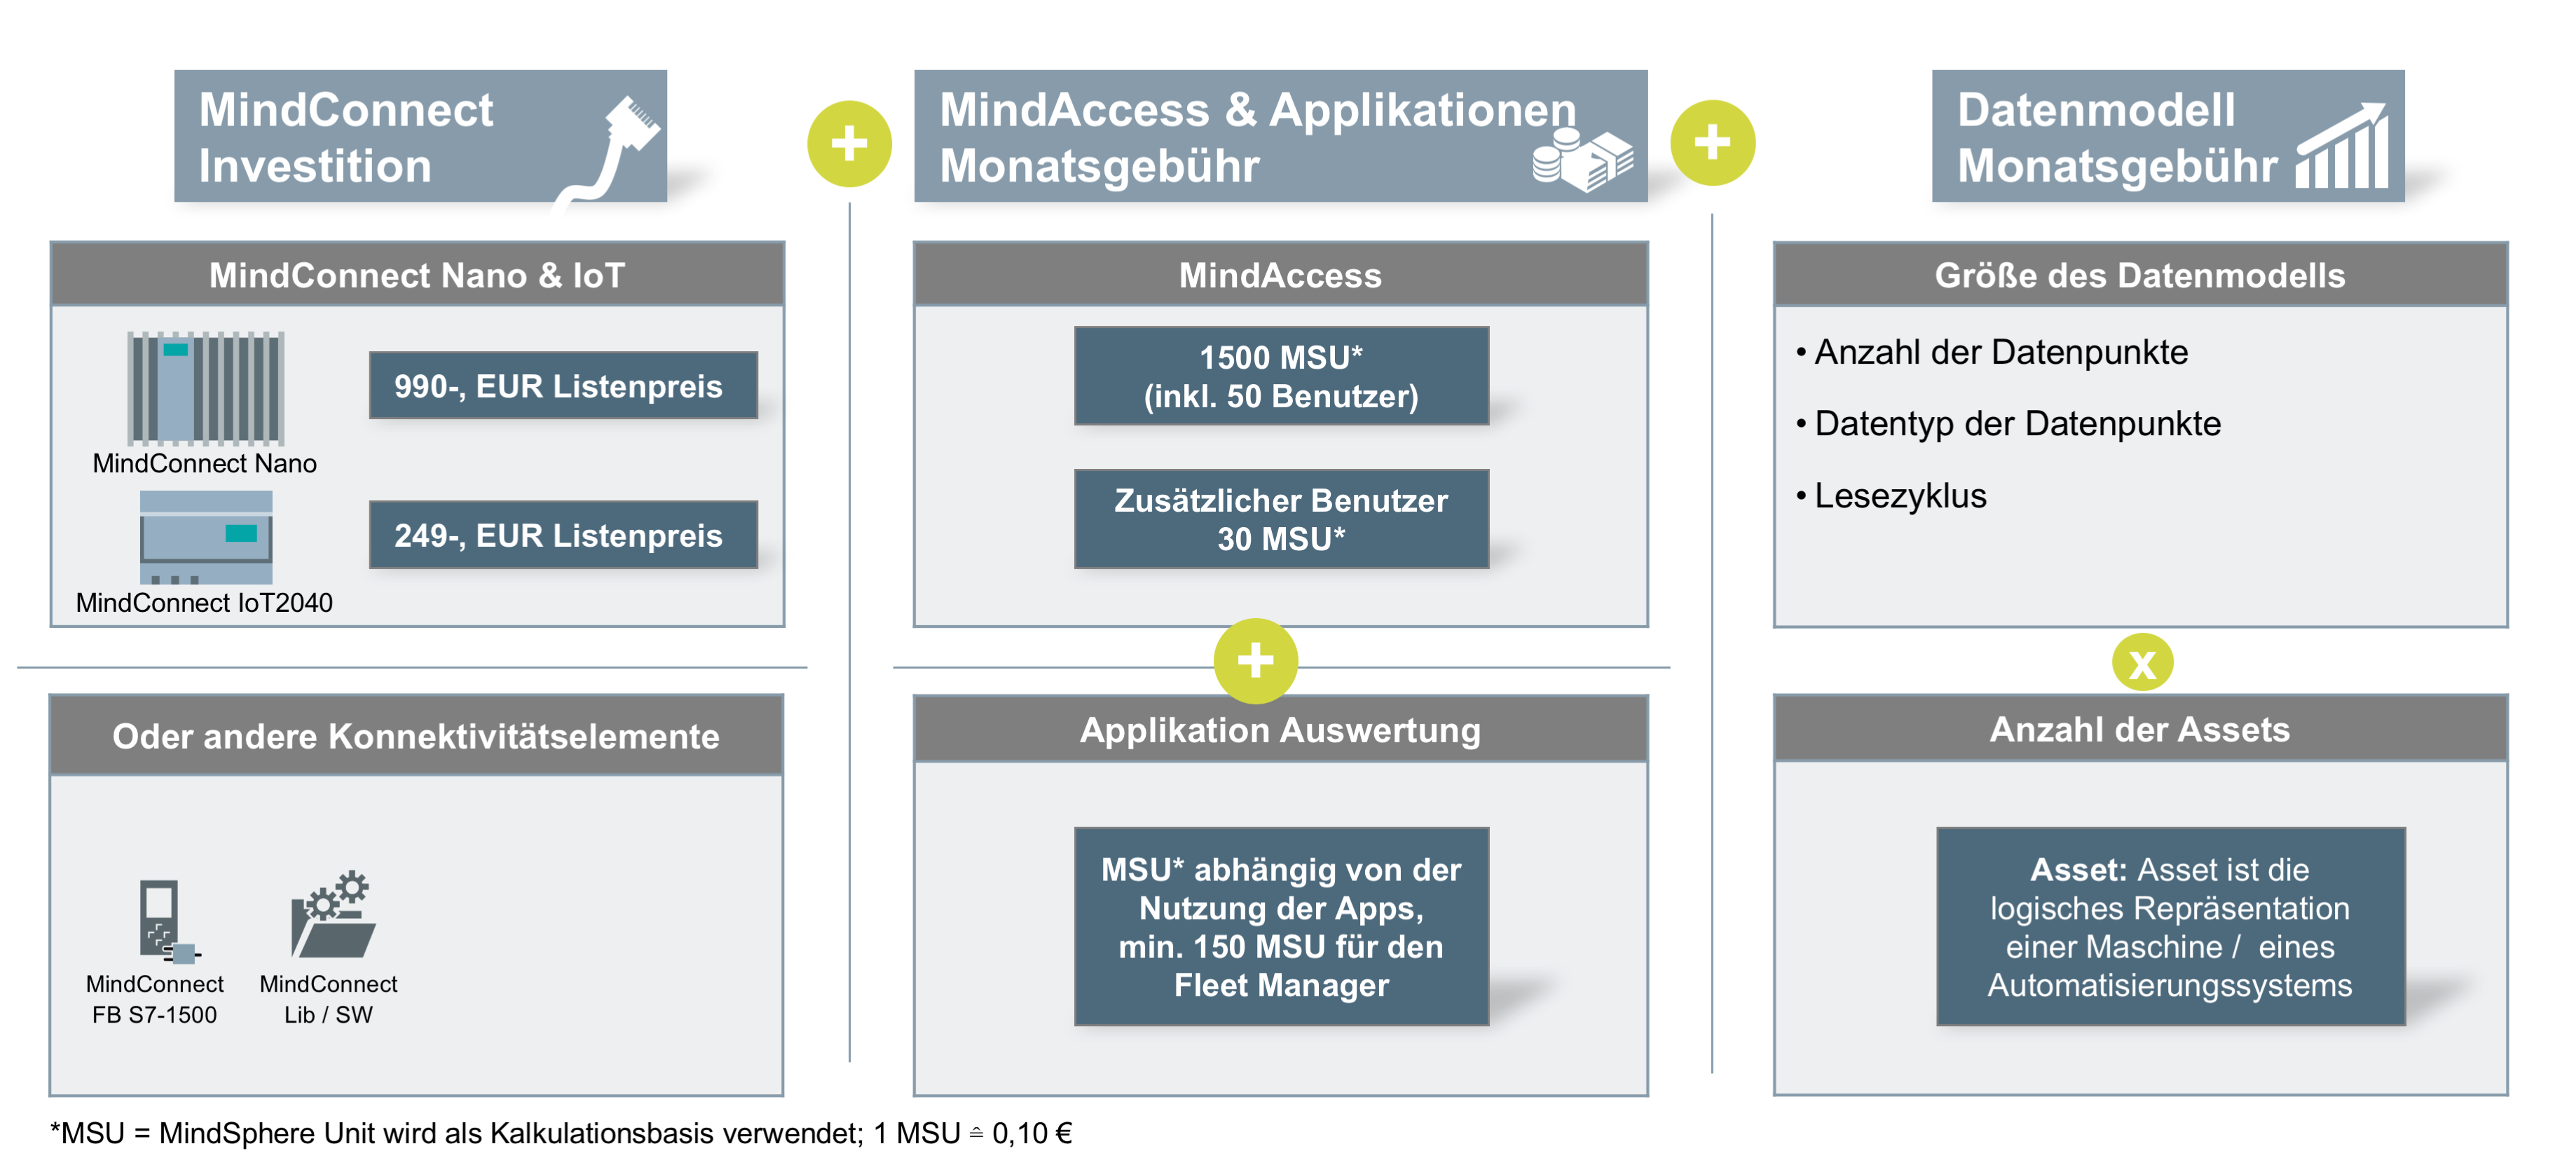
\includegraphics[width=1\textwidth]{PriceModel_1.png} 
\caption{Überblick über das MindSphere-Preismodell (vgl. \cite{SiemensMSIntroduction}).}
\label{fig:PriceModel}
\end{figure}















